%%%%%%%%%%%%%%%%%%%%%%%%%%%%%%%%%%%%%%%%%%%%%%%%%%%%%%%%%%%%%%%%%%%%%%%%%%%%%
%%
%% This file provides a template that can be used in concert with the
%% ohio-etd class to generate an electronic thesis or dissertation which
%% meets the formatting requirements at Ohio University.
%%
%% To use the template, copy this file (template.tex) and ohio-etd.cls into
%% the same directory and edit this template as required.  Reference
%% ohio-etd.pdf for additional instructions on using this class.
%%
%%%%%%%%%%%%%%%%%%%%%%%%%%%%%%%%%%%%%%%%%%%%%%%%%%%%%%%%%%%%%%%%%%%%%%%%%%%%%


%% Load the class.  Available options are: numbered, pdftex, cmfont,
%% singlespacetables, draft, 11pt, 12pt, leqno, and fleqn

\documentclass[numbered,pdftex]{ohio-etd}
\usepackage{cite}
\usepackage{notoccite}

\usepackage{ragged2e}
\usepackage{verbatim} 
\usepackage{hyperref}
\usepackage{flafter}
\usepackage{color,soul} % Highlighting 
\usepackage{subfigmat}

\usepackage{float} % In-text figs
\usepackage{varioref}%  smart page, figure, table, and equation ref
\usepackage{graphicx} % Include graphics
\usepackage{epstopdf} % Figure type .eps to .pdf
\usepackage{wrapfig} % Figures in text
\usepackage{listings}
\usepackage{color} %red, green, blue, yellow, cyan, magenta, black, white
\definecolor{mygreen}{RGB}{28,172,0} % color values Red, Green, Blue
\definecolor{mylilas}{RGB}{170,55,241}
%% Other packages that may be of use.  Delete or comment out (using a
%% percent sign in the first column) if they are not desired.  Reference
%% the corresponding documentation for more information on how to use these
%% packages.

%\usepackage[square,sort&compress,numbers]{natbib} % Provides formatting for
                                                  % citations
\usepackage{textcomp} % Provides math symbols that can be used in text mode
\usepackage{amssymb}  % Provides additional AMS math symbols.  Note that
                      % amsmath is loaded as part of the ohio-etd class
\usepackage{bm}       % Provides bold-faced math symbols
\usepackage{booktabs} % Provides improved table formatting
\usepackage{dcolumn}  % Provides table columns aligned at decimal points
\usepackage{multirow} % Provides table elements spanning multiple rows
\usepackage{graphicx} % Standard package to incorporate graphics
\usepackage[printonlyused]{acronym} % Provides a method for incorporating
                                    % acronyms and building an acronym list
\usepackage{relsize}
\usepackage{amsmath} % Inserting Equations

\graphicspath{{figures/}} % Allows graphics files to be stored in a
                          % separate directory
\usepackage{fancyref}
\usepackage{}

%% Required front matter definitions

\degree    {MS}              % MS, MA, MCTP, or PhD
\graduation{December}{2017}    % May, August, or December 

\title     {A Proposal for a Parameterized Circulating Vector Field Guidance for Fixed Wing Unmanned Aerial Vehicles}
\author    {Garrett S.}{Clem} 

\advisor   {Jay P. Wilhelm}{Assistant Professor of Mechanical Engineering}
\dean      {Dennis Irwin}{Dean, Russ College of Engineering and Technology }
\program   {Mechanical Engineering}            % e.g. Electrical Engineering
\department{Department of Mechanical Engineering} % e.g. School of Electrical Engineering 
                                    %      and Computer Science
\college   {Russ College of Engineering and Technology}   % e.g. Russ College of Engineering and
                                     %      Technology
\abstract  {ABSTRACT}


%% Optional front matter definitions.  Delete or comment out if not needed

% \coadvisor {Coadvisor's Full Name}{Coadvisor's Full Title}

\dedication{DED}

\acknowledgments{ACK}
%% If you prefer to provide "acknowledgements" instead (note the added "e"
%% between the "g" and the "m") then add the "e" in the macro name so that
%% it reads "\acknowledgements".}

%% Additional "lists" can be added to the end of the front matter using the
%% \addlistof macro.  For example:
\addlistof{Symbols}{\begin{tabbing}
  XXXX \= \kill% this line sets tab stop
  \\
  $a$ \> Previous or Initial Axial Induction Factor (-) \\
  

 \end{tabbing}}
%% Note that the command "\input{symbols}" can be used if the symbol list is
%% contained in a separate file called "symbols.tex"}

\addlistof{Acronyms}{

\begin{tabular}{lll}
AoA & Angle of Attack & \\
\end{tabular}}


%% Use "\input{acronyms}" if the acronym list is in a separate file called
%% "acronyms.tex".  Note that the formatting generated by the acronym package
%% can be forced into singlespaced text by inserting "\setlength\itemsep{0pt}
%% \setlength\parskip{0pt}" into the "acronym" environment.} 

%% For documents created by government employees as part of their
%% employment.  The wording of the disclaimer can be specified using an
%% option.  See the documentation for more information.

% \govtdisclaimer    

% \notables  % Prevent a list of tables from being created
% \nofigures % Prevent a list of figures from being created

\begin{document}

\makefrontmatter    % Creates all of the front matter pages.

% for matlab code entrys
\lstset{language=Matlab,%
    %basicstyle=\color{red},
    breaklines=true,%
    morekeywords={matlab2tikz},
    keywordstyle=\color{blue},%
    morekeywords=[2]{1}, keywordstyle=[2]{\color{black}},
    identifierstyle=\color{black},%
    stringstyle=\color{mylilas},
    commentstyle=\color{mygreen},%
    showstringspaces=false,%without this there will be a symbol in the places where there is a space
%     numbers=left,%
%     numberstyle={\tiny \color{black}},% size of the numbers
%     numbersep=6pt, % this defines how far the numbers are from the text
    emph=[1]{for,end,break},emphstyle=[1]\color{red}, %some words to emphasise
    %emph=[2]{word1,word2}, emphstyle=[2]{style},    
}

%% Body of the text follows, using \chapter, \section, \subsection,
%% \subsubsection, \paragraph, and \subparagraph to generate the
%% section headings.  For convenience, it may be useful to break the
%% full document into separate files, perhaps divided by chapters.  In
%% that case, the files would be loaded here using "\input{filename}"


\chapter{Introduction}
\section{Motivation and Problem Statement}
% Fixed wing Unmanned Aerial Vehicles are used for  missions such as surveillance and reconnaissance that might put pilots harms way \cite{bone_uavs_2003}. UAVs carry out mission objectives such as waypoint navigation and loitering by following paths that are typically pre-planned \cite{sujit_unmanned_2014}. Known obstacles are avoided during the planning processes to avoid collisions. Paths must be of obstacles which may not be known during planning. Obstacles are not always known during planning and once discovered a new path may have to be re-planned. Guidance that follows mission paths while avoiding obstacles without the need for re-planning may be beneficial. Gradient vector field (GVF) guidance is a path following method that provides continuous guidance that guaranteed to converge and follow an arbitrary path. Guidance for getting on and following a path is produced by summing together convergence and circulation terms that are weighted by static scalars. Obstacles have been represented as separate repulsive GVFs that are later summed to the path following GVF [Wilhelm, Wambold, Clem]. Static GVFs do not always route the UAV around an obstacle and could be improved. Modifying the GVF convergence and circulation weights to be functions of common UAV states could be used to produce an optimal guidance for obstacle avoidance. \textbf{The proposed research seeks to determine GVF weighting functions that construct optimal obstacle avoidance.}
% \pagebreak
Fixed wing Unmanned Aerial Vehicles are used for missions such as surveillance and reconnaissance that might put pilots harm’s way \cite{bone_uavs_2003}. Missions consist of sequential objectives that are represented by a path that the UAV attempts to follow. Paths are typically pre-planned before flight and are constructed by connecting straight lines and circular arcs. Vehicle turn rate constraints and obstacles are considered when planning a path to prevent collisions or entry into no-fly zones. UAVs are guided to follow a path by implementing guidance algorithms which calculate headings that minimize the distance to a path. UAVs may encounter an obstacle whose position was previously unknown while following a pre-planned path which may require a new path to be generated. Guidance that follows mission paths while avoiding obstacles without the need for re-planning may be beneficial. 
\\
Gradient Vector Field (GVF) guidance is a path following method that has been adapted for obstacle avoidance. GVFs produces continuous heading vectors that guide a UAV to converge and follow a path by summing together convergence and circulating terms that are weighted by static scalars. An obstacle represented as a path and given a negative convergence weight results in a repulsive field that can be used for obstacle avoidance. Static GVFs do not always route the UAV around an obstacle and could be improved. Modifying the GVF convergence and circulation weights of obstacle fields to be functions of common UAV states could be used to produce an optimal guidance for obstacle avoidance. \textbf{The proposed research seeks to determine GVF weighting functions that construct optimal obstacle avoidance.}


 \pagebreak
 
 
\section{Methods Overview}
The proposed research will be conducted in three phases where VF guidance  singularities will be demonstrated, weighting functions will be investigated, and a developed GVF will be validated on a ground robot simulating a UAV.  Phases I and II will be conducted in a simulation environment that combines mission paths and obstacles into a single GVF. Phase III will be conducted with a ground robot simulating a UAV guided by the modified GVF in real-time. Dubin's fixed wing constraints will be imposed in simulations and experiments. 


\section{Phase I}
\textbf{Recreate gradient vector fields for circular and elliptical obstacles and demonstrate singularities.} A simulation environment will be built that generates GVFs consisting of mission paths and obstacles. Circular and elliptical obstacles will be investigated and the resulting singularities will be characterized. Static weights will be used and the performance of the guidance measured in distance traveled and time of flight. 



\section{Phase II}
\textbf{Investigate GVF weighting functions that influence obstacle avoidance.} UAV closing rate, position, and range will be used to develop dynamic GVF weights for convergence and circulation. The modified GVF will be compared against a static and strictly repulsive GVF. Distance traveled and time of flight will be used to as metrics to compare the modified GVF to the unmodified GVF.  



\section{Phase III}
\textbf{Validate modified GVF model with ground robot experiments.} The modified GVF developed in Phase II will be implemented on a differential drive ground robot simulating a fixed wing UAV. Guidance performance while avoiding static obstacles will be demonstrated.
 

\section{Summary of Phases}

Each phase consists of an \textbf{objective} that will be accomplished by executing \textit{tasks}.
 Completion of all objectives and phases will result in the final \underline{deliverable}. \\[1cm]

\noindent
\textbf{Phase I:} Demonstrate Gradient Vector Field Singularities
\textit{
\begin{enumerate}
	\item Build a GVF simulation environment
	\item Derive GVF for circular and elliptical obstacles
	\item Identify path and obstacles where singularities are produced 
\end{enumerate}
}

\noindent
\textbf{Phase II:} Investigate GVF weighting functions that influence obstacle avoidance
\textit{
\begin{enumerate}
	\item Formulate circulation and convergence weights as functions of UAV state
	\item Determine combination of GVF weights that produces optimal guidance in simulation
\end{enumerate}
}

\noindent
\textbf{Phase III:} Validate modified GVF model with ground robot experiments
\textit{
\begin{enumerate}
	\item Build differential drive robot
	\item Build robotic framework to take guidance commands
	\item Repeat simulations performed in Phase II on ground robot
\end{enumerate}
}

\noindent
\textbf{Deliverable:} \underline{Adaptive GVF parameterized weights optimal guidance for path following and static} \underline{ obstacle avoidance}.





\chapter{Literature Review}
\section{Introduction to Literature Review}


\section{Unmanned Aerial Vehicle}

Unmanned Aerial Vehicles (UAVs) are pilotless aircraft used by military, police, and civilian communities for tasks such as surveillance, reconnaissance, damage assessment, and natural disaster surveying.  UAVs are generally categorized into fixed wing and rotor craft varieties that range in size, payload, and flight time capabilities. The aircrafts can be controlled remotely with a RC transmitter or fly on pre-planned paths executing maneuvers such as waypoint navigation and loitering. Data can be collected with on-board sensors such as cameras which then can be stored or relayed to the ground. UAVs are part of an Unmanned Aerial System (UAS) which is made up of the vehicle, autopilot, ground station, transmitter, and two way radio which is depicted in Figure \ref{fig:uas}. Ground stations are responsible for monitoring the vehicle's status, planning missions, and generating obstacle free and flyable paths which are sent to the autopilot via two way radio. 

\begin{figure}
	\centering
	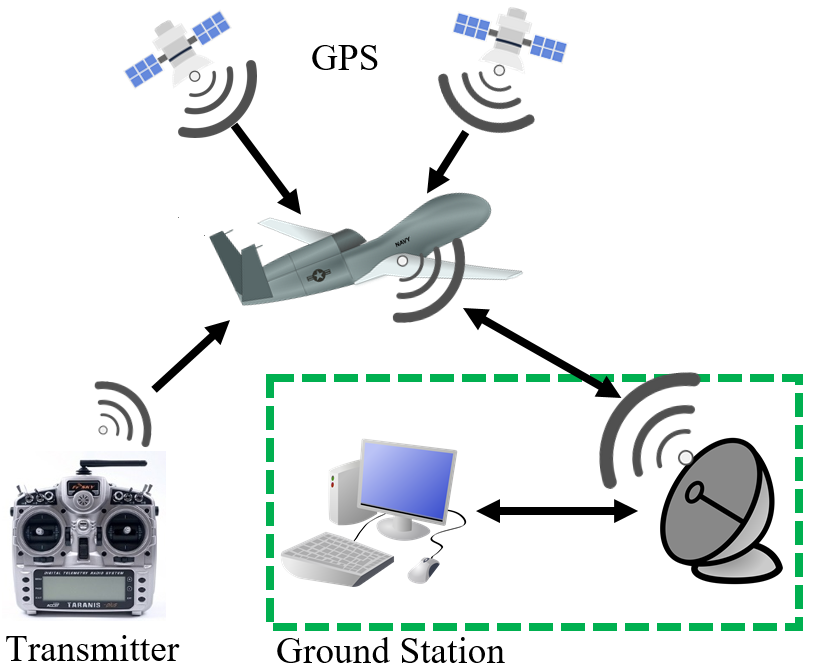
\includegraphics[width=8cm]{PaperFigures/UAS}
	\caption{Unmanned Aerial System (UAS)}
	\label{fig:uas}
\end{figure}

The autopilot is responsible for following the pre-planned path and maintaining vehicle stability while under the influence of external wind disturbances. Stable flight while path following is accomplished by implementing feed-back control, navigation, and guidance systems. Feed-back refers to the closure of an open-loop control system which allows an error to be calculated between the desired state of the UAV, the reference, and the current state of the UAV. Reference error is used to calculate the necessary actuator output required to modify the vehicles attitude and position while preventing unbounded osculations. Feed-back is provided by the navigation system which uses sensors to measure the attitude and position of the aircraft. Sensors often provide noisy data and are sampled at varying rates. Filtering and estimation techniques such as the Kalman filter which fuses and filters measurements to provide an improved state estimation. A high level overview of the autopilots systems can be seen in Figure \ref{fig:autopilotloops}.

\begin{figure}
	\centering
	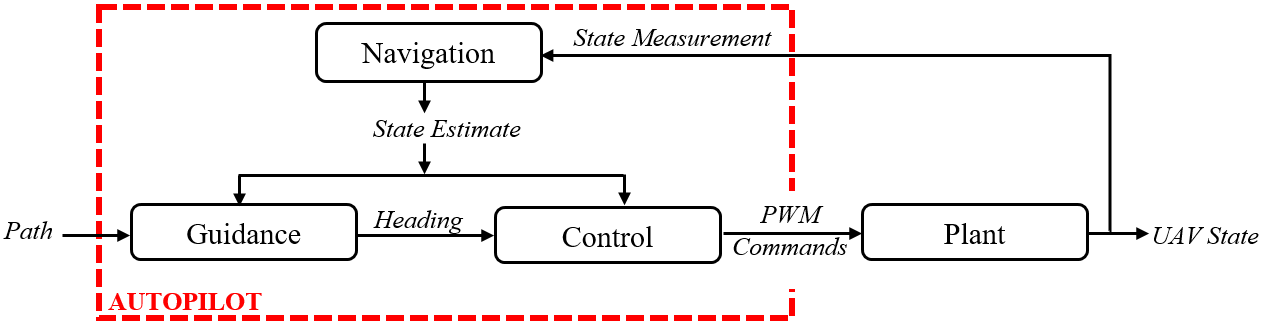
\includegraphics[width=15cm]{PaperFigures/autopilotLoops}
	\caption{Autopilot's Navigation, Guidance, and Control Architecture}
	\label{fig:autopilotloops}
\end{figure}

The navigation system is responsible for taking high level pre-planned paths from the ground station and providing a reference heading command to the control system. Several methods for path following guidance were investigated in \cite{sujit_unmanned_2014} consisting of carrot chasing, non-linear guidance law, pure line-of-sight, linear quadratic regulator, and gradient vector field method. A Monte Carlo simulation with wind disturbances was conducted for the guidance methods above in \cite{sujit_unmanned_2014}. It was determined that the vector field method followed the path with least tracking error and control effort which is the primary goal of path following. 


\section{Vector Field Guidance}

\subsection{Introduction to Vector Field Guidance}
Vector field is a continuous guidance and control method that applies artificial attractive and repulsive forces to a point mass. The two broad categories of algorithms that produce vector fields consist of potential field algorithms and path following algorithms. Potential field produces guidance and control to a robot for converging to a distinct point. Path following algorithms produce guidance for converging and following a path. Several path following vector field algorithms have been investigated including gradient vector field, which provides convenient convergence and circulation weights that may be useful for providing an optimal guidance for obstacle avoidance. 

%Intro (what are vector fields and what are they used for)
%Two types
%PF
%Path following
%Gradient vector field is good

\subsection{Potential Field}

%%%%%%%%%%
Potential field was introduced as a real-time robotic manipulator algorithm for obstacle avoidance \cite{khatib_real-time_1986}. The potential field algorithm represents a robots workspace as a gradient potential of attractive and repulsive artificial forces that drive the robot to a desired goal. Goals are given the lowest potential and act as attractive forces. Obstacles have high potential and act as repulsive forces. A simple example is depicted in Figure \ref{fig:pfobstacle} consisting of an initial state, a goal, and a single obstacle. The initial state of the robot is at the edge of a gradient where the potential is maximum. In the lowest part of the gradient a goal exists at the global minimum. Obstacles are added to the potential field, but have limited effect due to a decay function.

\begin{figure}[h!]
	\centering
	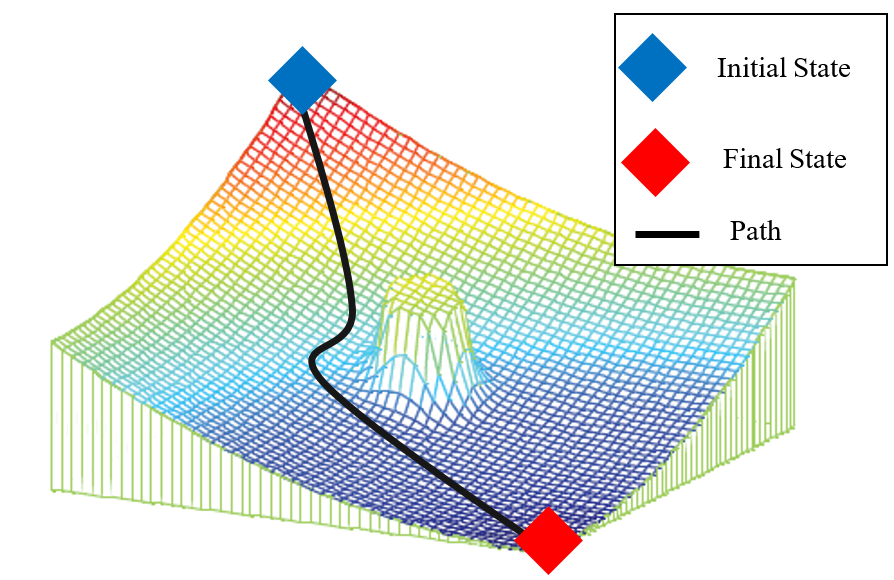
\includegraphics[width=7cm]{PaperFigures/pfObstacle}
	\caption{Single Obstacle Potential Field Gradient \cite{liu_virtual-waypoint_2016}}
	\label{fig:pfobstacle}
\end{figure}

Potential field is unique in that path planning, trajectory planning, and control are lumped into a single system \cite{rimon_exact_1992}. Transition from an initial state to a goal state traditionally occurred by executing three steps consisting of path planning, trajectory planning, and control. Path planning dealt with finding an obstacle free path from an initial state to a goal state. Trajectory planning time parametrized the obstacle free path with some high level vehicle constraints considered. Lastly, control attempts to reduce the tracking error with respect to the reference trajectory. Combining the three motion planning steps into a single algorithm has been shown to be computational inexpensive \cite{goerzen_survey_2010}. 

As pointed out in \cite{borenstein_real-time_1990}, robots using potential field are susceptible to local minimum. Encountering a local minimum prevents the robot from continuing down the gradient and into the global minimum because equilibrium has been reached prematurely. Figure \ref{fig:pfLocalMin} demonstrates local minimum by adding several obstacles into a goal field. Several methods have been developed to mitigate the effects of local minimums as pointed out in \cite{goerzen_survey_2010} through the use of navigation functions. Local minimum produced as a result of closely spaced obstacles as shown in Figure \ref{fig:pfLocalMin} have been addressed by grouping obstacles together into a cluster \cite{liu_virtual-waypoint_2016}.

\begin{figure}[h]
	\begin{subfigmatrix}{2}% number of columns
		\centering
		\subfigure []{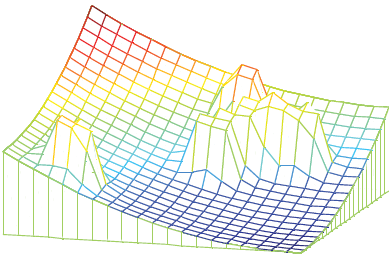
\includegraphics[width=7cm] {PaperFigures/pfObstacleLocalMin}}
		\subfigure []{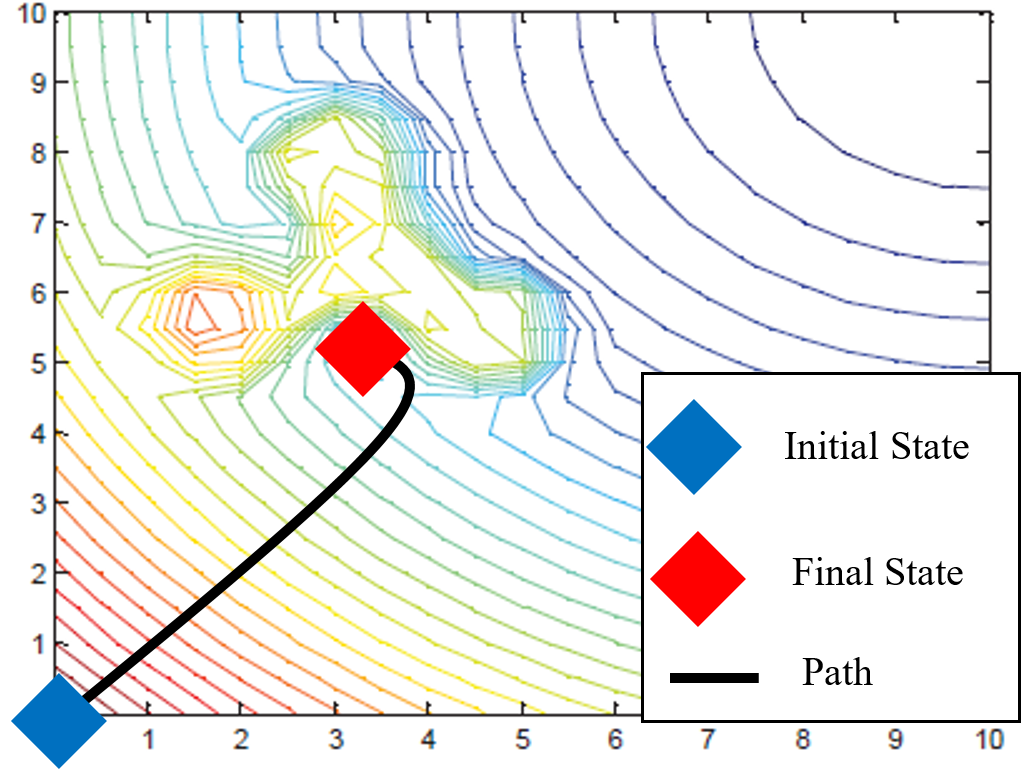
\includegraphics[width=7cm] {PaperFigures/pfObstacleLocalMinTopology}}
		%		\hspace*{1cm}
	\end{subfigmatrix}
	\caption{Potential Field Local Minimum \cite{liu_virtual-waypoint_2016}}
	\label{fig:pfLocalMin}
\end{figure}

Several methods have been developed to mitigate the effects of local minimums as pointed out in \cite{goerzen_survey_2010} through the use of navigation functions. Local minimum produced as a result of closely spaced obstacles as shown in Figure \ref{fig:pfLocalMin} have been addressed by grouping obstacles together into a cluster \cite{liu_virtual-waypoint_2016}. Grouping obstacles addresses the risk of local minima before forming the potential field. If local minima are encountered after the field is generated, additional forces can be applied to push the robot away from the local minima. 

\begin{figure}[H]
	\centering
	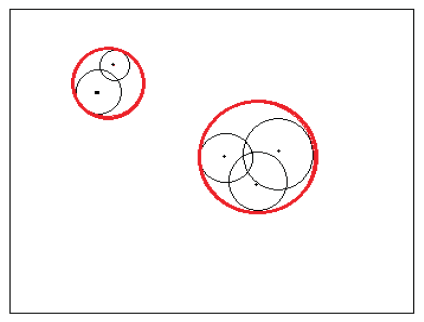
\includegraphics[width=5cm]{PaperFigures/obstacleClustering}
	\caption{Obstacle Clustering \cite{liu_virtual-waypoint_2016}}
	\label{fig:obstacleclustering}
\end{figure}

Potential fields ability to avoid obstacles and combine path planning, trajectory planning, and control into a single system while being computationally inexpensive makes it an attractive option for many robotic systems. Fixed wing UAVs must maintain a minimum forward velocity and cannot converge to a single point, making potential field difficult to implement. 

%%%%%%%%%%%%%%%%%%%%%%%%%%%%%%%%%%%%%%%%%%%%%%%%%%%%%%%%%%%%%%%%%%%%%%%%%%%%%%%%%%%%%%%




%%%%%%%%%%%%%%%%%%%%%%%%%%%%%%%%%%%%%%%%%%%%%%%%%%%%%%%%%%%%%%%%%%%%%%%%%%%%%%%%%%%%%%%


\subsection{Virtual Force Field - Histogram Method}
When the environment changes, such as a new obstacle or the goal has moved, the potential field has to be recalculated. Koren and Borenstein developed a virtual force field (VFF) histogram method that guides a mobile robot to a known goal while avoiding initially unknown obstacles \cite{borenstein_real-time_1990}. VFF decomposes a robots workspace into discretized cells that contain an integer certainty value associated with the confidence that an obstacle occupies the cell. A global goal applies an artificial attractive force on the robot that pulls it closer to the goal. As the robot detects obstacles, the certainty value increases in the cell associated with the obstacles position. Cells apply artificial repulsive forces with magnitudes that depend on the certainty value and the distance to the cell. 

\begin{figure}
	\centering
	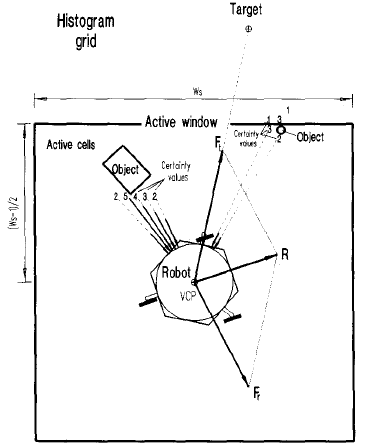
\includegraphics[width=7cm]{PaperFigures/histogram}
	\caption{Virtual force field histogram acting on a mobile robot}
	\label{fig:histogram}
\end{figure}


The VFF histogram method was validated on a mobile robot platform using ultrasonic sensors in \cite{borenstein_real-time_1990} and \cite{borenstein_vector_1991}, avoiding obstacles and seeking a goal. Certainty cells in VFF only provide strictly repulsive vectors which guide the robot away, but provide no guidance for getting around the obstacle. 
 
 
%%%%%%%%%%%%%%%%%%%%%%%%%%%%%%%%%%%%%%%%%%%%%%%%%%%%%%%%%%%%%%%%%%%%%%%%%%%%%%%%%%%%%%%
 
 
 
 
%%%%%%%%%%%%%%%%%%%%%%%%%%%%%%%%%%%%%%%%%%%%%%%%%%%%%%%%%%%%%%%%%%%%%%%%%%%%%%%%%%%%%%%
 
\subsection{Lyapunov Vector Fields}

Fixed wing UAVs must maintain a minimum forward velocity therefore cannot converge to a single point making potential field or VFF guidance difficult. Missions for UAVs are typically constructed from obstacle free paths build from straight line and circular arc primitives. Path planning provides a reference to the autopilot that guides the UAV to first arrive at and subsequently follow the desired path while under the influence of external disturbances. 
Ariving at and following the path are typically is typically achieved by generating vectors normal and parallel to the path respectively. Nelson et al. introduced a vector field generation method for straight line and circular arcs using Lyapunov stability arguments \cite{nelson_cooperative_2005} and is depicted in Figure \ref{fig:nelsonlyapunov}.

\begin{figure}
	\centering
	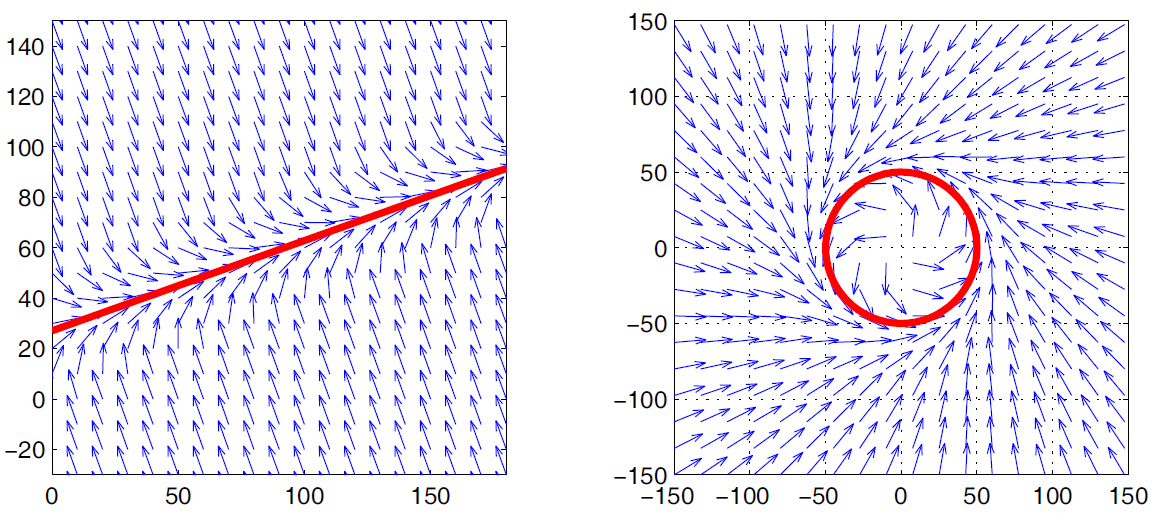
\includegraphics[width=13cm]{PaperFigures/nelsonLyapunov}
	\caption{Lyapunov vector field for straight line and circular primitives}
	\label{fig:nelsonlyapunov}
\end{figure}

To construct flyable paths out of the primitives, it was necessary to determine how the resulting vector fields should be combined. Summing the fields directly result in \hl{deadzones, sinks, and singularities}. The solution was to have a single field active at any time, switching when the UAV reached the end of a primitive. Nelson's method was extended by Griffiths for curved path following and showed that the vectors asymptotically approach the curved path, shown in Figure \ref{fig:griffiths}.

\begin{figure}
	\centering
	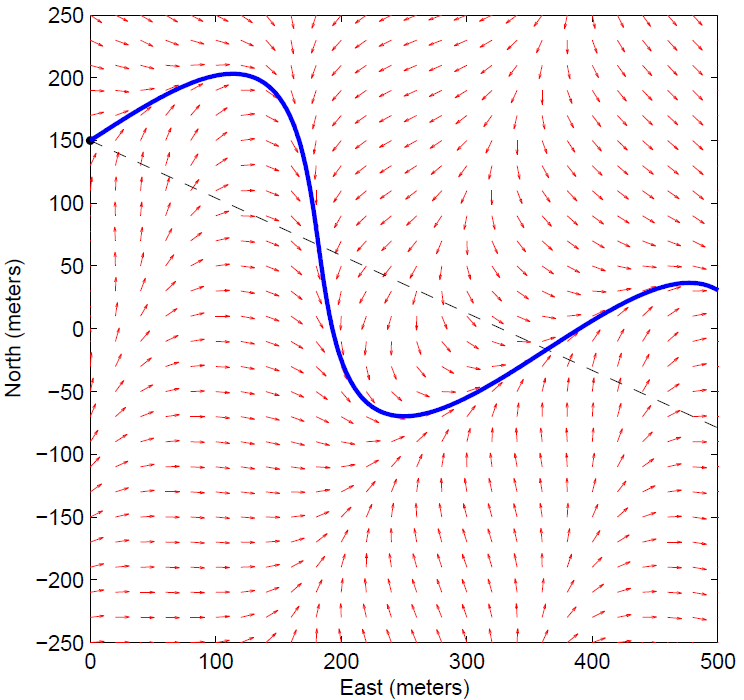
\includegraphics[width=7cm]{PaperFigures/griffiths}
	\caption{Lyapunov vector field approach curved path asymptotically}
	\label{fig:griffiths}
\end{figure}


Primitive circular fields can be modified via non-linear coordinate transformations to produce globally convergent elliptical fields \cite{frew_lyapunov_nodate}\cite{frew_cooperative_2007}. Frew simulated and experimentally validated the transformed vector field where multiple fixed wing UAVs cooperatively tracked a moving target while maintaining a staggered distance from each other, preventing collision and multiple surveillance angles. The location of a target being tracked is not known with absolute certainty. The covariance matrix from a kalman filter to transform a circular vector field around an uncertain target was investigated in \cite{frew_cooperative_2007} and an example field is shown in Figure \ref{fig:lyapunovFrew}b.

\begin{figure}[h]
	\begin{subfigmatrix}{2}% number of columns
		\centering
		\subfigure []{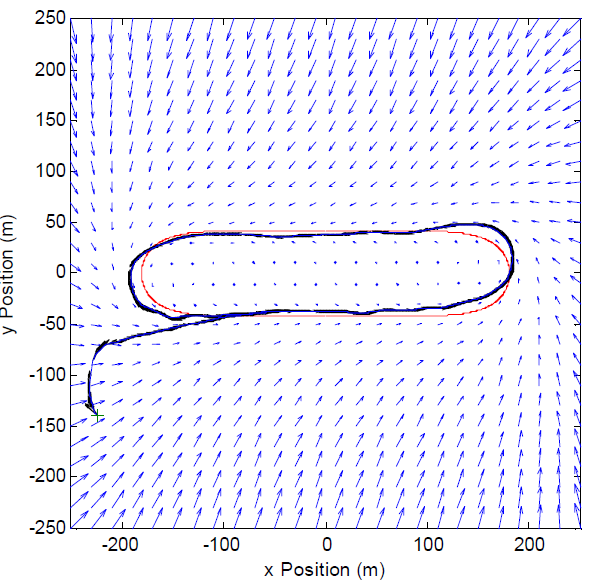
\includegraphics[width=6.25cm] {PaperFigures/lyapunovFrew}}
		\subfigure []{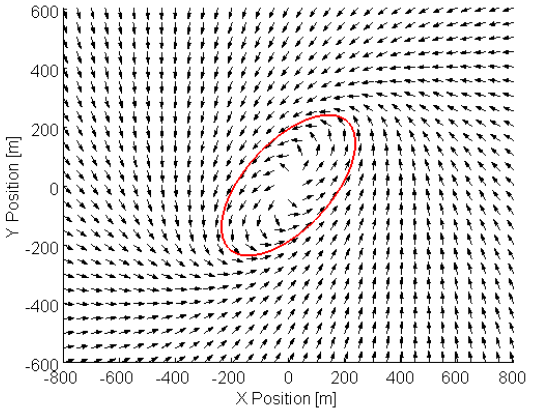
\includegraphics[width=8cm] {PaperFigures/lyapunovFrewUncertain}}
		%		\hspace*{1cm}
	\end{subfigmatrix}
	\caption{Elliptical VF produced by non-linear coordinate transformations a)\cite{frew_lyapunov_nodate} b)\cite{frew_cooperative_2007}}
	\label{fig:lyapunovFrew}
\end{figure}

A target tracking lyapunov plus tangent vector field was introduced in \cite{chen_tracking_2009} that produced shorter paths compared to lyapunov alone. Outside of the standoff circle, tangent vectors were said to provide the shortest distance to the circle. Inside the standoff circle, no tangent lines exist and lyapunov is used in its place. Figure \ref{fig:lyapunovChen} shows the difference in paths taken for lyapunov and tangent vector fields outside the standoff circle. The TPLVF was later used for path planning to avoid obstacles in \cite{chen_uav_2013}.

\begin{figure}
	\centering
	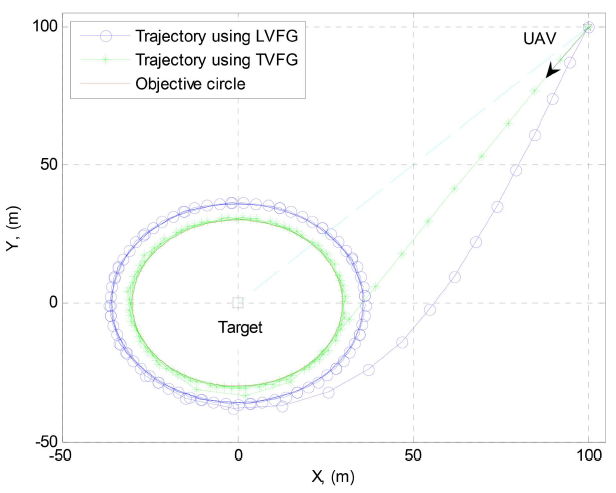
\includegraphics[width=7cm]{PaperFigures/lyapunovChen}
	\caption{Tangent plus lyapunov vector fields for shortest path target tracking \cite{chen_uav_2013}}
	\label{fig:lyapunovChen}
\end{figure}


\subsection{Non-Lyapunov Vector Fields}

All methods that consider obstacles so far build a vector field that guides the UAV to an obstacle free path. Another approach is to build a vector field tending to a path and use optimal rapid random trees (RRT*) to explore the space for obstacles and select the optimal path. Pereia et al. developed such a method that builds a tree that makes up possible paths for the UAV to take. Branches extend from the root, or initial location of the UAV, randomly throughout the map with a constrained deviation from the initial vector field. When a branch encounters an obstacle it is trimmed and no longer explored. The path of minimum cost, or least distance, is selected for the UAV to use as a reference path. An example of the algorithm is shown in Figure \ref{fig:rrtvf}.

\begin{figure}
	\centering
	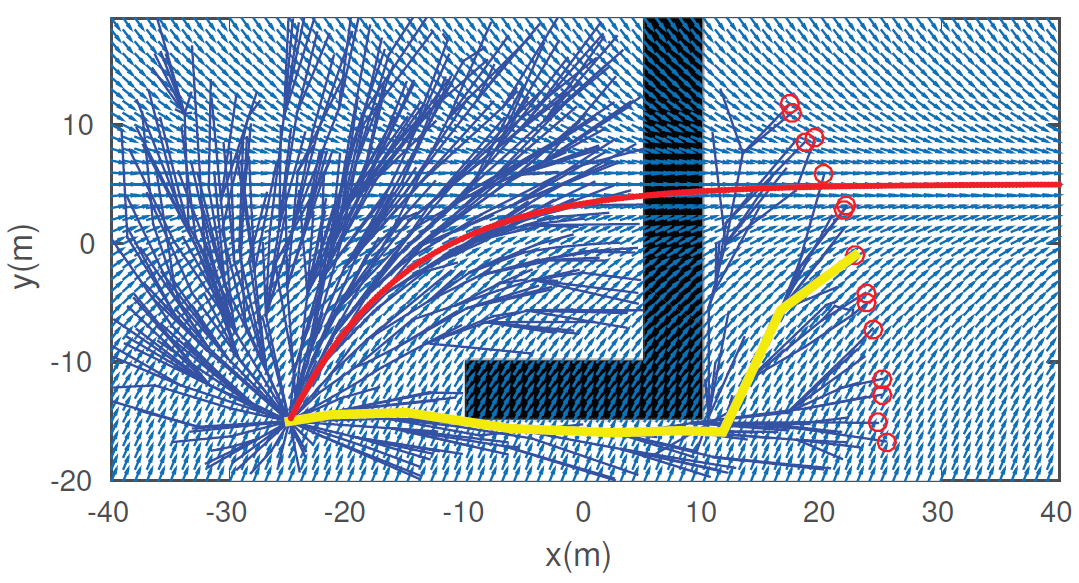
\includegraphics[width=12cm]{PaperFigures/rrtVF}
	\caption{RRT* path planner with a VF used as a task specification}
	\label{fig:rrtvf}
\end{figure}


For well known obstacles in urban environments, such as buildings, an optimal path can be constructed with constrained delaunay triangulation (CDT) which has been previously used in computer animation \cite{md_simplex_2017}. CTD was used to construct vector fields in \cite{pimenta_fully_2007} that restricts robots movements inside the triangles while moving towards a global goal. A simulation of a robot traversing a vector field inside a set of CDTs can be seen in Figure \ref{fig:cdtVF}.

\begin{figure}
	\centering
	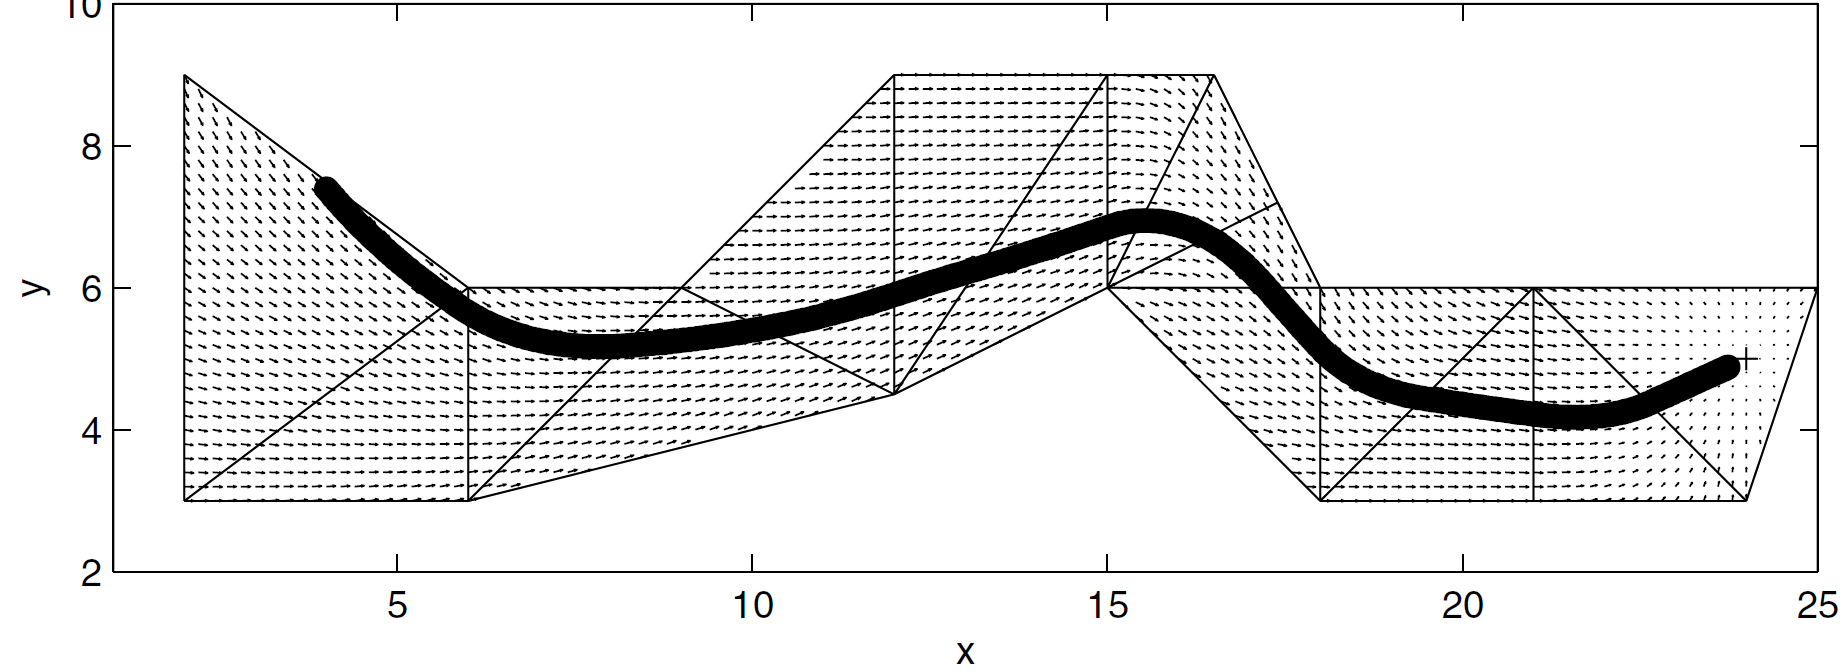
\includegraphics[width=15cm]{PaperFigures/cdtVF}
	\caption{Vector field within a set of constrained delaunay triangles \cite{pimenta_fully_2007}}
	\label{fig:cdtVF}
\end{figure}


So far all of the vector field methods discussed have avoided obstacles by planning paths around them. Paths are typically calculated at the ground station and if communication is lost a new path may not be relayed to a UAV encountering a new obstacle. A possible solution is using vector fields to provide a repulsive force, not unlike the VFF method, immigrating around the obstacle. 



% = = = = = = = = = = = = = = = = = = Think about using something like this in the literature review summary
%So far vector fields built from straight line and circular primitives that are commonly used by path planners to construct missions have been discussed. The method used to build primitives can be extended to construct vector fields that asymptotically converge to curved paths.  Primitives can be modified with coordinate transforms to construct racetrack and elliptical shapes for target following of moving and uncertain targets. Obstacles can be avoided through RRT* that uses a vector field to sense the general direction of branch expansion, and a robotic system can maintain a collision free path inside of a set of constrained triangles with vector fields.

\subsection{Gradient Vector Field}
The gradient vector field method was first introduced in \cite{goncalves_artificial_2009} and produces an $n$-dimensional vector field guaranteed to converge to a path made of points that lie at the intersection of two surfaces. The total vector field $\vec{V}$ is produced by summing together a convergence, circulation, and time varying terms seen in Equation \ref{gonFieldeq}. Convergence terms contribute vectors normal to the path, circulation terms contribute vectors parallel to the path, and time varying vectors account for changes in the path as a function of time. 

\begin{equation}
% Component vector field with conv and circ
\vec{V} = \boldsymbol{G}\vec{V}_{conv} + \boldsymbol{H}\vec{V}_{circ} +  \boldsymbol{L}\vec{V}_{tv} 
\label{gonAllComp}
\end{equation}

Each term is multiplied by a scalar, \textit{\textbf{G}}, \textit{\textbf{H}}, \textit{\textbf{L}}, that weights the contribution of each term on the total field $\vec{V}$. Only static paths will be discussed so it is assumed the time varying field is null. The advantage of GVF is the convenient access to the weighting terms that independently effect the total field. Magnitude of the weights modifies the strength of each fields influence, whereas the sign indicates the direction. Figure \ref{fig:positiveUnity} shows convergence and circulation fields for a circular path where the weights \textit{\textbf{G}} and \textit{\textbf{H}} are unity and positive. The convergence field contains vectors that are normal to the circular path for all points in space, with exception to the center of the circle which is undefined. Circulation fields contain vectors that are parallel to the path for all points in space with the same exception of no definition at the center of the circle. 

\begin{figure}[]
	\begin{subfigmatrix}{2}% number of columns
		\centering	
		\subfigure []{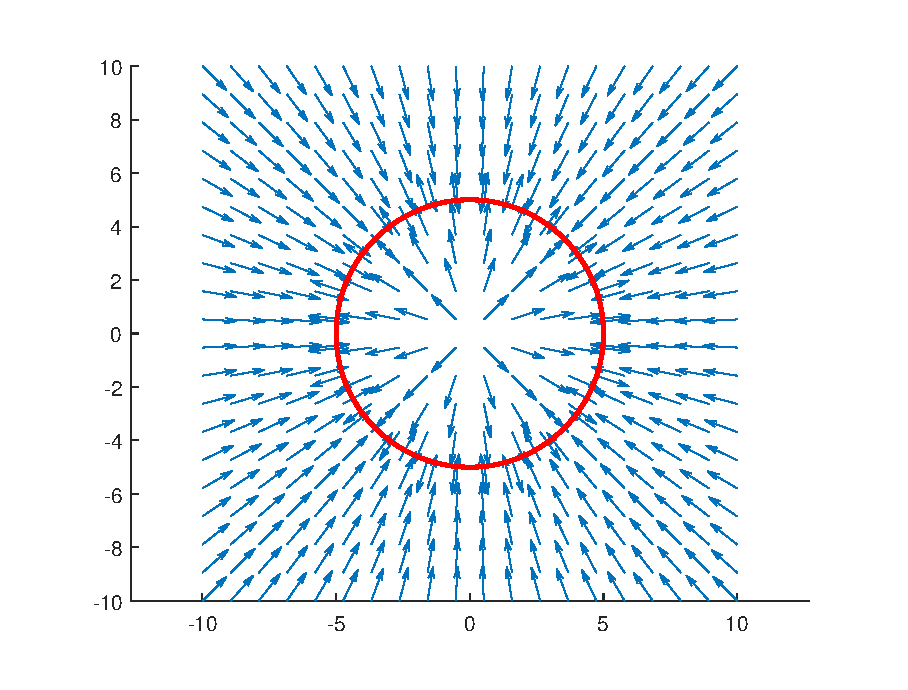
\includegraphics[width=7.5cm] {PaperFigures/gFieldOnly}}
		\subfigure []{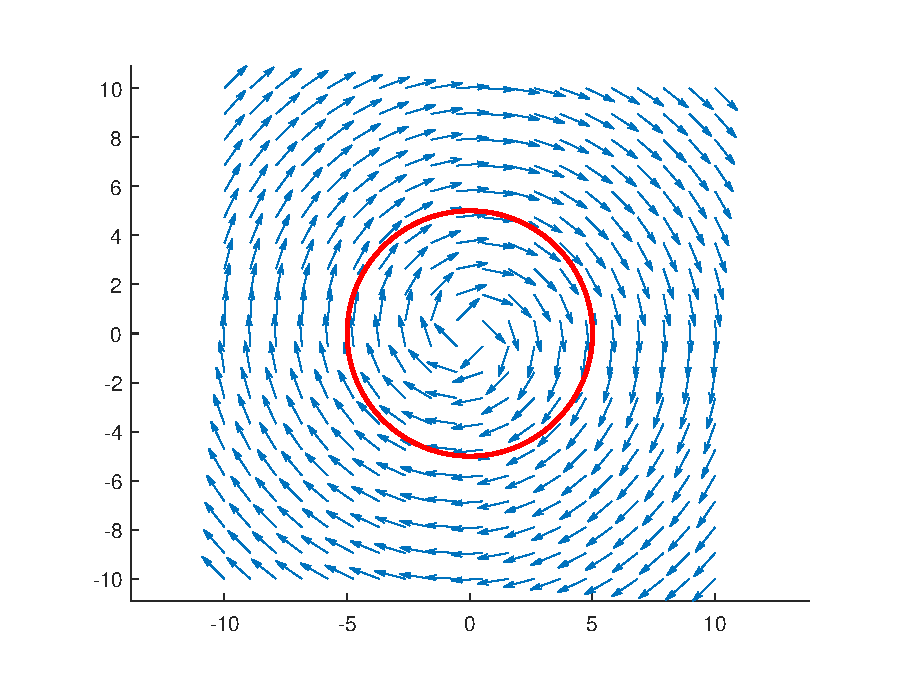
\includegraphics[width=7.5cm] {PaperFigures/hFieldOnly}}
		\hspace*{0mm}
	\end{subfigmatrix}
	\caption{Attractive vector field (a) and clockwise circulation field (b)}
	\label{fig:positiveUnity}
\end{figure}

Modifying the signs of \textit{\textbf{G}} and \textit{\textbf{H}} to be unity and negative results in similar fields but with a $180^{\circ}$ rotation about the center of the circle, Figure \ref{fig:negativeUnity}. The attractive convergence field becomes a repulsive field, where all vectors are anti-normal to the path. The circulation field changes direction and rotates counterclockwise around the path. 

\begin{figure}[]
	\begin{subfigmatrix}{2}% number of columns
		\centering	
		\subfigure []{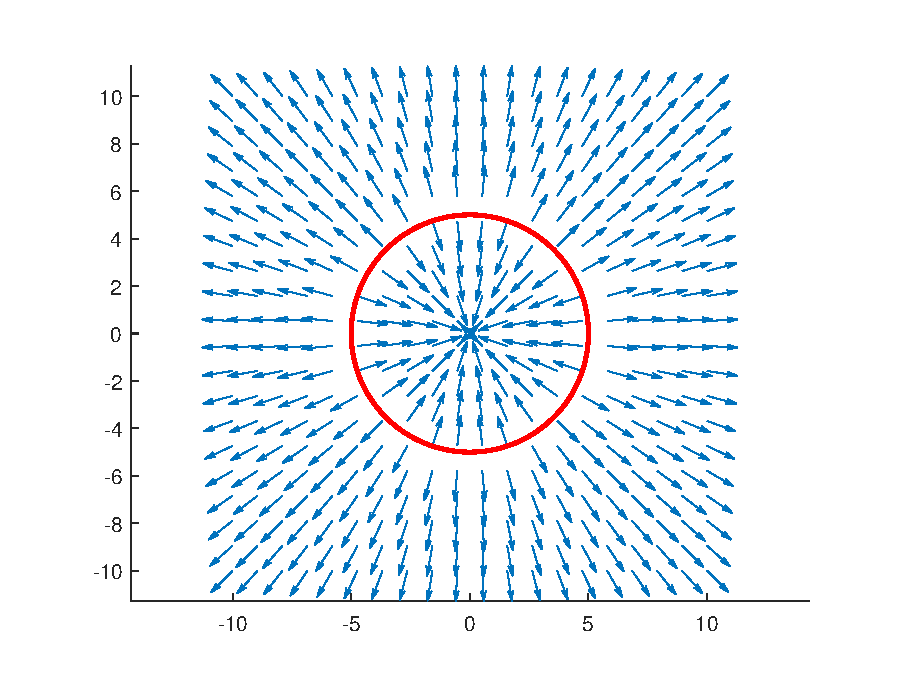
\includegraphics[width=7.5cm] {PaperFigures/_gFieldOnly}}
		\subfigure []{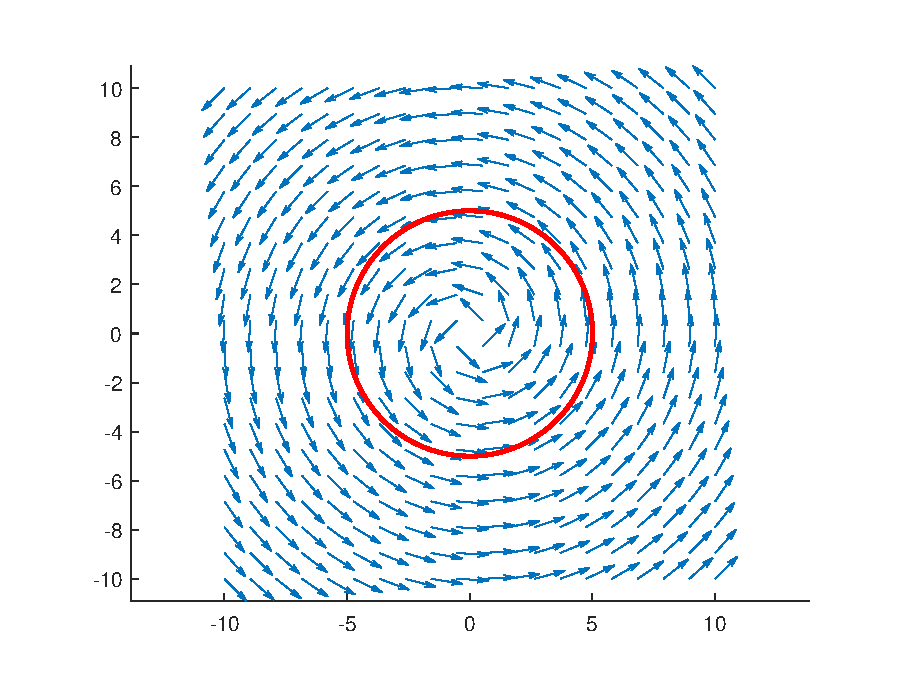
\includegraphics[width=7.5cm] {PaperFigures/_hFieldOnly}}
		\hspace*{0mm}
	\end{subfigmatrix}
	\caption{Repulsive vector field a) and counterclockwise circulation field b)}
	\label{fig:negativeUnity}
\end{figure}

Repulsive fields have been used for obstacle avoidance for a UAV loitering around a moving target in [w,w,c]. A circular goal path was attached to a ground vehicle and a convergence and circulation vector field was generated. Circular paths were with small radii were placed on top of obstacles with strictly repulsive weights. Notice in Figure \ref{fig:negativeUnity}a that inside of the path, vectors guide inward, which is not desired for obstacle avoidance. The problem is aleviated by reducing the radius significantly. Goal and obstacle field are summed together to provide a total field that provides guidance to a UAV. Loitering is accomplished while avoiding two obstacles, as shown in Figure  \ref{fig:gvfMovingTarget} 

\begin{figure}[h]
	\centering
	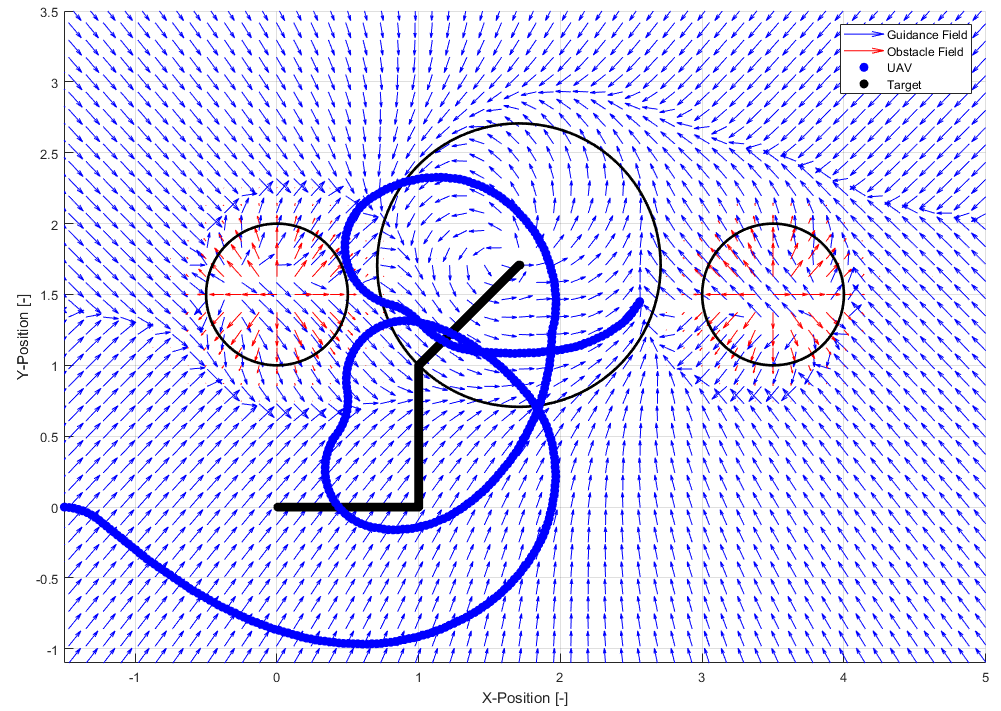
\includegraphics[width=7cm]{PaperFigures/gvfMovingTarget}
	\caption{Place holder image of UAV following ground target}
	\label{fig:gvfMovingTarget}
\end{figure}


Similar to potential field and VFF, the strength of the repulsive field depends on the distance from an obstacle. In [w,w,c], a tangent hyperbolic decay function was assigned to the obstacle fields which varied the total strength from null to unity, shown in Figure \ref{fig:tanhICUAS2018}. 

\begin{figure}
	\centering
	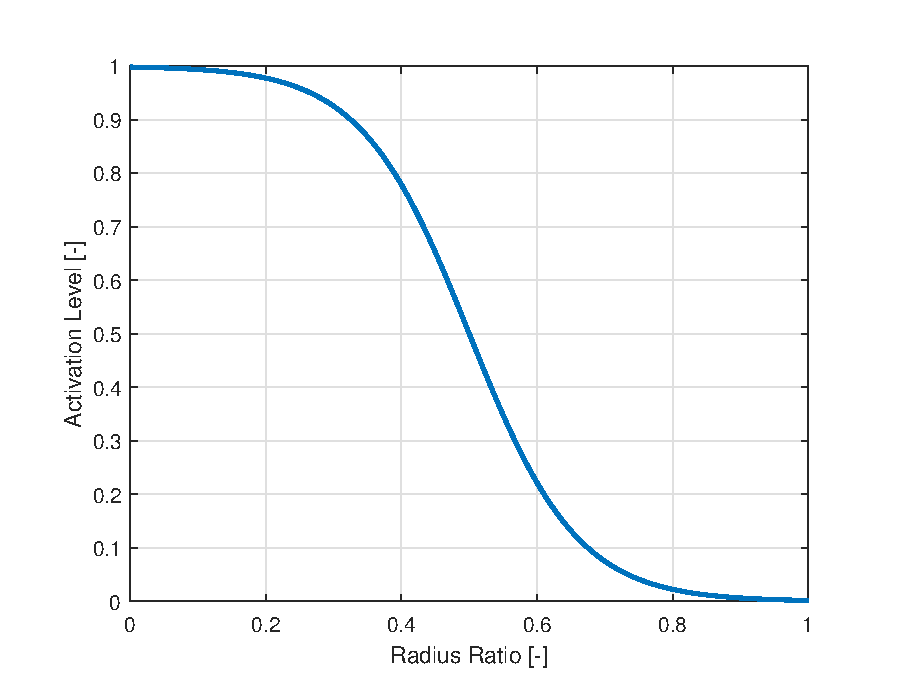
\includegraphics[width=10cm]{PaperFigures/tanh_ICUAS2018}
	\caption{}
	\label{fig:tanhICUAS2018}
\end{figure}



Constructing the paths for a UAV flying at constant altitude requires three-dimensional surfaces intersecting to form two-dimensional paths. Consider a UAV in 2-dimensional space tracking a path $\tau$, which is made of points that lie at the intersection of two surfaces. Each of the surfaces $\alpha_i$ is continuous, differentiable, and is a function of the set $q = [x,y,z]$. The convergence field $\vec{V_{conv}}$ is produced by the sum of surfaces multiplied by their respective partial gradient $\nabla_q\alpha_i$. The definition of the convergence field is summarized in Equations \ref{convOnly} and \ref{partials}.



\begin{equation}
% Total field with Conv, Circ, and Time
\vec{V}_{conv} = \boldsymbol{G}\sum_{i=1}^{n-1}\alpha_i\nabla_q\alpha_i  
\label{convOnly}
\end{equation}

\begin{equation}
\label{partials}
\nabla_q=\begin{bmatrix}
\frac{\partial}{\partial x} \\
\frac{\partial}{\partial y} \\
\frac{\partial}{\partial z}
\end{bmatrix}
\end{equation}

To produce a circular path of radius $r$ the intersection of a cylinder and plane are used, as shown in Equations \ref{cylinder}-\ref{plane} and pictured in Figure \ref{fig:cylinderPlane}.

\begin{figure}
	\centering
	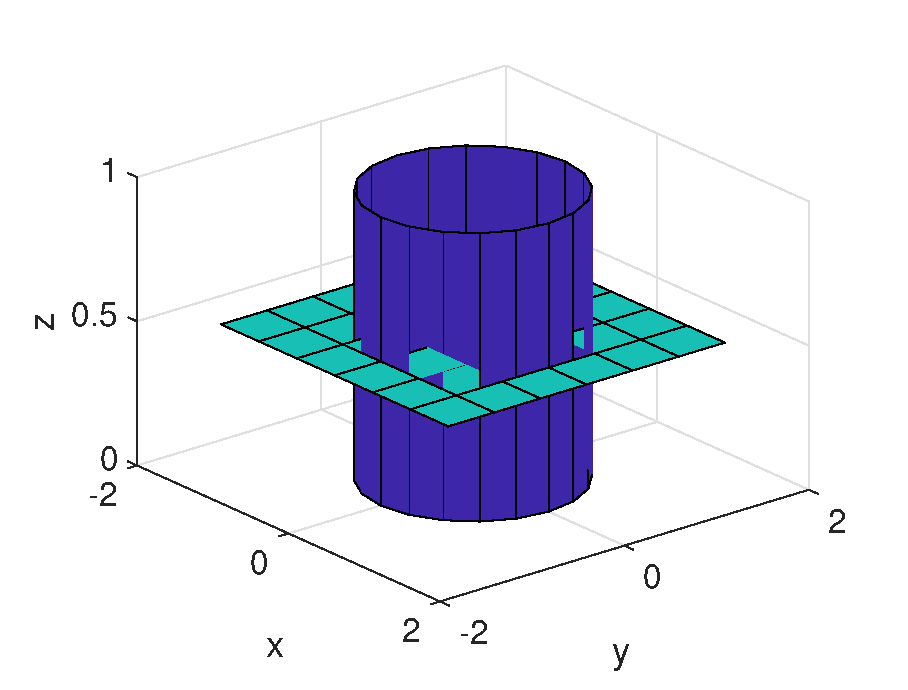
\includegraphics[width=7cm]{PaperFigures/cylinderPlane}
	\caption{}
	\label{fig:cylinderPlane}
\end{figure}

\begin{equation}
\label{cylinder}
\alpha_1 = x^2+y^2-r
\end{equation}

\begin{equation}
\label{plane}
\alpha_2 = z
\end{equation}

Convergence vector field term is produced by taking the wedge product of the partials $\nabla_q\alpha_i$, which in three dimensions simplifies to the cross product as shown in Equations \ref{circOnly} and \ref{circOnlySimp}.


\begin{equation}
% Total field with Conv, Circ, and Time
\vec{V}_{circ} =  \boldsymbol{H}\wedge_{i=1}^{n-1}\nabla_q\alpha_i 
\label{circOnly}
\end{equation}

\begin{equation}
% Total field with Conv, Circ, and Time
\vec{V}_{circ} =  \boldsymbol{H}(\nabla_q\alpha_1 \times \nabla_q\alpha_2) 
\label{circOnlySimp}
\end{equation}


Circulation and convergence terms may have different magnitudes depending on the location of origin of a vector and the equations used for surfaces. Normalizing each component prior to weighting allows for more predictable results when assigning values. So far the VF weights have been used for high level specification of the desired behavior for a UAV, whether it be for convergence, avoidance, or circulation. Furthermore, there is no guarauntee that when using a vector field for avoidance that the UAV will not violate the no-fly zone. If the UAV turn rate is at saturation an increased reference command will do nothing to aid in avoidance. A demonstration of saturation is seen in Figure \ref{fig:inputSat} where a UAV is provided guidance by a convergent and circulating vector field about a circular path. 

\begin{figure}
	\centering
	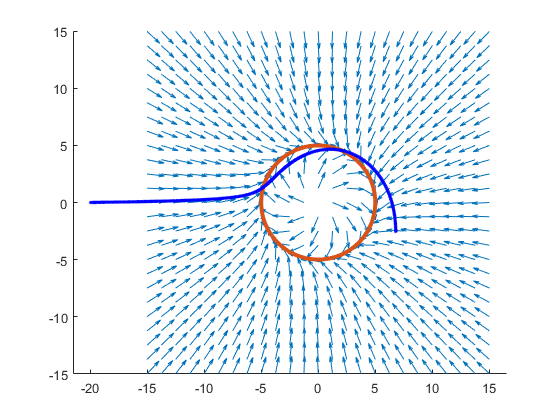
\includegraphics[width=12cm]{PaperFigures/inputSat}
	\caption{Dubins UAV actuator saturation}
	\label{fig:inputSat}
\end{figure}

If the VF was adjusted earlier at an earlier state, the tracking error may be reduced. When using an obstacle, determining which direction the UAV must fly around the obstacle is important to reduce distance flown. Determining functions for the sign and magnitude of the vector field weights to produce an optimal guidance.

%${[x_1,x_2,\cdots,x_n]^T \in \!R} : $
%$\alpha_i(x_1,x_2,. . .,x_n)$
%$(i=1,2,...,n-1)$
%\begin{equation}
%% Total field with Conv, Circ, and Time
%\vec{V} = \boldsymbol{G}\sum_{i=1}^{n-1}\alpha_i\nabla_q\alpha_i  +  \boldsymbol{H}\wedge_{i=1}^{n-1}\nabla_q\alpha_i   +  \boldsymbol{L}M^{-1}a
%\label{gonFieldeq}
%\end{equation}

%\begin{equation}
%% Component vector field with conv and circ
%\vec{V} = \boldsymbol{G}\vec{V}_{conv} + \boldsymbol{H}\vec{V}_{circ} 
%\label{gonComp}
%\end{equation}


%\begin{equation}
%%Spatial dimensions of gon vf
%q = [x_1,x_2,...x_n]
%\label{gonDims}
%\end{equation}




%	\begin{itemize}
%		\item VF in literature have guided/followed paths that have been pre-defined
%		\item Intersection of surfaces, zero sets represent path
%		\item n-dimensions for any shapes (unlike some Lyapunov made of primitives)
%		\item Guaranteed vectors converge to path
%		\item Equations (convergence, circulation, tv)
%		\item Obstacles and paths are static, TV term is not considered
%		\item Examples of components FIGURES: (circulation,convergence,total)
%		\item Normalization of vectors gives each component equal influence on the total vector
%		\item After normalization a scalar weight influences how much influence each component has
%		\item Weights do not effect the guarantee of convergence (non zero and positive)
%		\item FIGURE: With normalization, without normalization (SIDE BY SIDE)
%		\item Dubins vehicle example of saturation
%		\item Static GVF weights do not consider state of the vehicle and provide sub-optimal guidance for obstacle avoidance
%		%Last Point to make
%		\item \hl{Dynamic GVF weights as a function of vehicle state may provide an optimal guidance for obstacle avoidance}
%\end{itemize}



\section{Unmanned Aerial Vehicle Simulation}
Testing new guidance, navigation, and control algorithms can be costly, require significant time, and requires an adequately large airspace. Ground stations need to be established which require power and shelter. Some small fixed wing UAVs may not be suitable to fly in all weather, therefore test flights may be canceled due to weather conditions. Lastly, larger UAVs need to have FAA clearance before flight which has to be pre-approved and takes time. Before spending the time to reserve airspace and allocate man hours for flight tests it is important to test algorithms in a controlled environment. One way to accomplish testing without actual flight is through validation through mobile robots simulating fixed wing constraints \cite{ren_experimental_2007}, \cite{louali_designing_2014}, \cite{louali_experimental_2016}. Programming a mobile robot, such as one shown in Figure

\begin{figure}
	\centering
	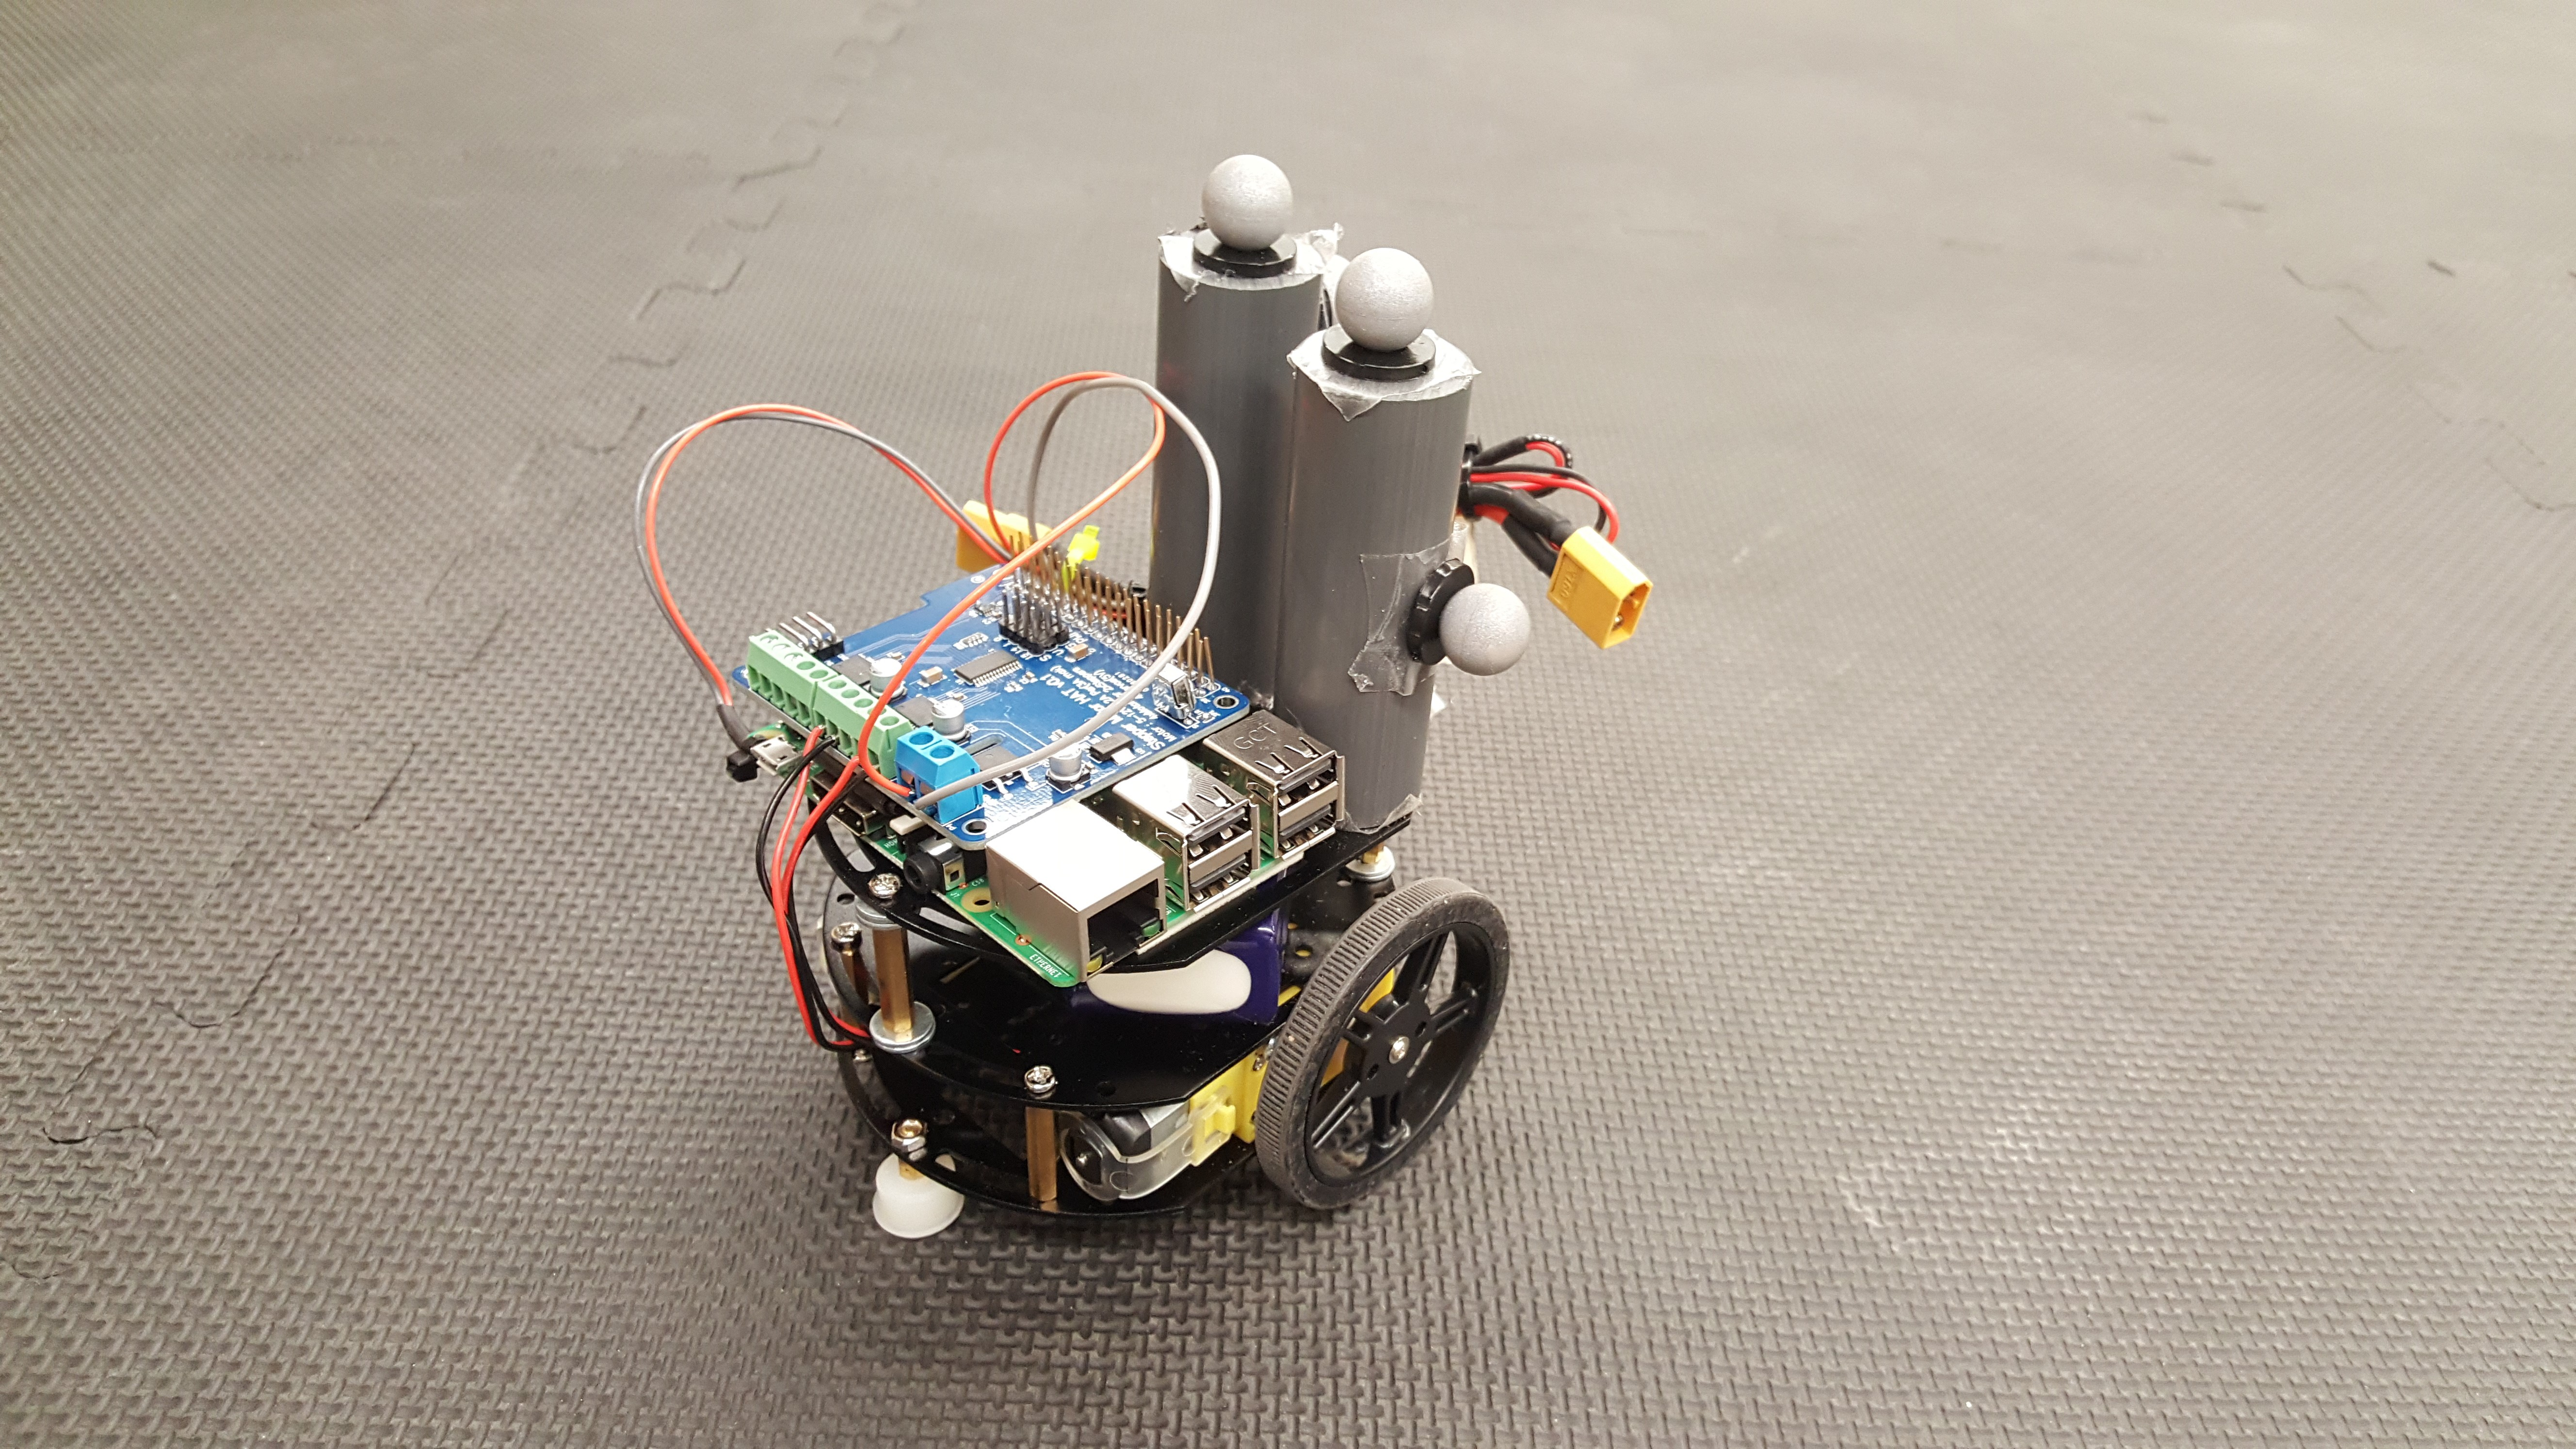
\includegraphics[width=12cm]{PaperFigures/robot}
	\caption{Differential drive mobile robot simulating fixed wing UAV Dubins constraints}
	\label{fig:robot}
\end{figure}


%\begin{itemize}
%	\item Methods for testing UAVs
%	\item SITL
%	\item Actual flight tests
%	\item Testing UAVs costly, setup, environment difficulties
%	\item Simulation on ground robot (citations)
%	\item Benefits, use as Dubins constraint vehicle to prove algorithm can run real time prior to flights
%	\item Less expensive, saves resources, time, etc
%\end{itemize}

\section{Literature Review Summary}

\begin{itemize}
	\item 
\end{itemize}

\bibliographystyle{aiaa}   
\bibliography{bib}


\end{document}
























%%%%%%%%%%%%%%%%%%%%%%%%%%% Old Literature Review Material

%
%
%\chapter{Literature Review}
%\section{Introduction to Literature Review}
%
%% The following sections provide a discussion on the literature in regards to the modeling of fixed wing UAVs and the navigation, guidance, and control systems that govern the behavior of the crafts
%% 
%%
%
%The following sections provide a discussion on the literature in regards to the modeling of fixed wing UAVs and the navigation, guidance, and control systems that govern the behavior of the crafts. First, the fixed wing is introduced and a brief discussion on the modeling techniques commonly used for navigation, guidance, and control design. An overview of the structure of autopilots that execute the models is presented. Then, an overview of navigation, guidance, and control is given along with the cutting edge techniques for guidance. (Revisit this section when a rough draft is complete)
%
%
%\section{Fixed Wing Unmanned Aerial Vehicle}
%\subsection{Introduction to Fixed Wing UAV}
%%  Fixed wing UAVs have found significant use in surveillance and reconnaissance in hostile environments since no on-board pilot is required.
%%  UAVs can be sent missions and piloted remotely, keeping soldiers out of harms way
%%  Operators can be relieved easily when becoming fatigued without landing the UAV, allowing it to fly for extended missions, accomplishing more tasks
%%  Fixed wings come in many different sizes and configurations but can be categorized into large and hand lanched varieties
%%  Large fixed wing UAVs require long stretches of runway to takeoff and land, are gas powered, and can carry large payloads consisting of sensor packages, high resolution cameras, and scientific instrumentation shown in Figure \ref{fig:globalhawk}.
%
%Fixed wing UAVs have been used for surveillance and reconnaissance in hostile environments since no on-board pilot is required. Ground stations allow for remote data collection and piloting, keeping soldiers out of harms way. During long endurance missions, operators can easily be changed out when fatigued allowing the UAV to remain in service for many hours beyond what a single pilot could safely handle. Keeping the UAV in service for longer allows more tasks to be accomplished. Fixed wing UAVs come in many different sizes and configurations, but can be categorized into large and hand-launched varieties. Large fixed wing UAVs require long stretches of runway to takeoff and land, are gas powered, and can carry large payloads consisting of sensor packages, high resolution cameras, and scientific instrumentation shown in Figure \ref{fig:fixedwings}a. Hand-launched UAVs can be easily broken down and carried by a single person and are often battery powered. Easily deployed, the hand-launched UAVs take-off by being thrown in a similar way as a javelin shown in Figure \ref{fig:fixedwings}b. The smaller form factor makes hand-launched UAVs well suited for short range reconnaissance and for carrying lightweight payloads with low to medium resolution cameras.
%
%%Fixed wing UAVs have found uses in surveillance, reconnaissance, environmental surveying, aerial photography, and competitive racing. The crafts are well suited to carry out tasks that require long endurance and large payloads.
%%Fixed wing UAVs come in many different sizes and configurations, but can be categorized into large and hand-launched varieties. Large fixed wing UAVs require long stretches of runway to takeoff and land, are gas powered, and can carry large payloads consisting of sensor packages, high resolution cameras, and scientific instrumentation shown in Figure \ref{fig:globalhawk}. Hand-launched UAVs can be easily broken down and carried by a single person and are often battery powered. Easily deployed, the hand-launched UAVs take-off by being thrown in a similar way as a javelin shown in Figure \ref{fig:handlaunched}. The smaller form factor makes hand-launched UAVs well suited for short range reconnaissance and for carrying lightweight payloads with low to medium resolution cameras. \\
%
%\begin{figure}[H]
%	\begin{subfigmatrix}{2}% number of columns
%		\centering
%		\subfigure []{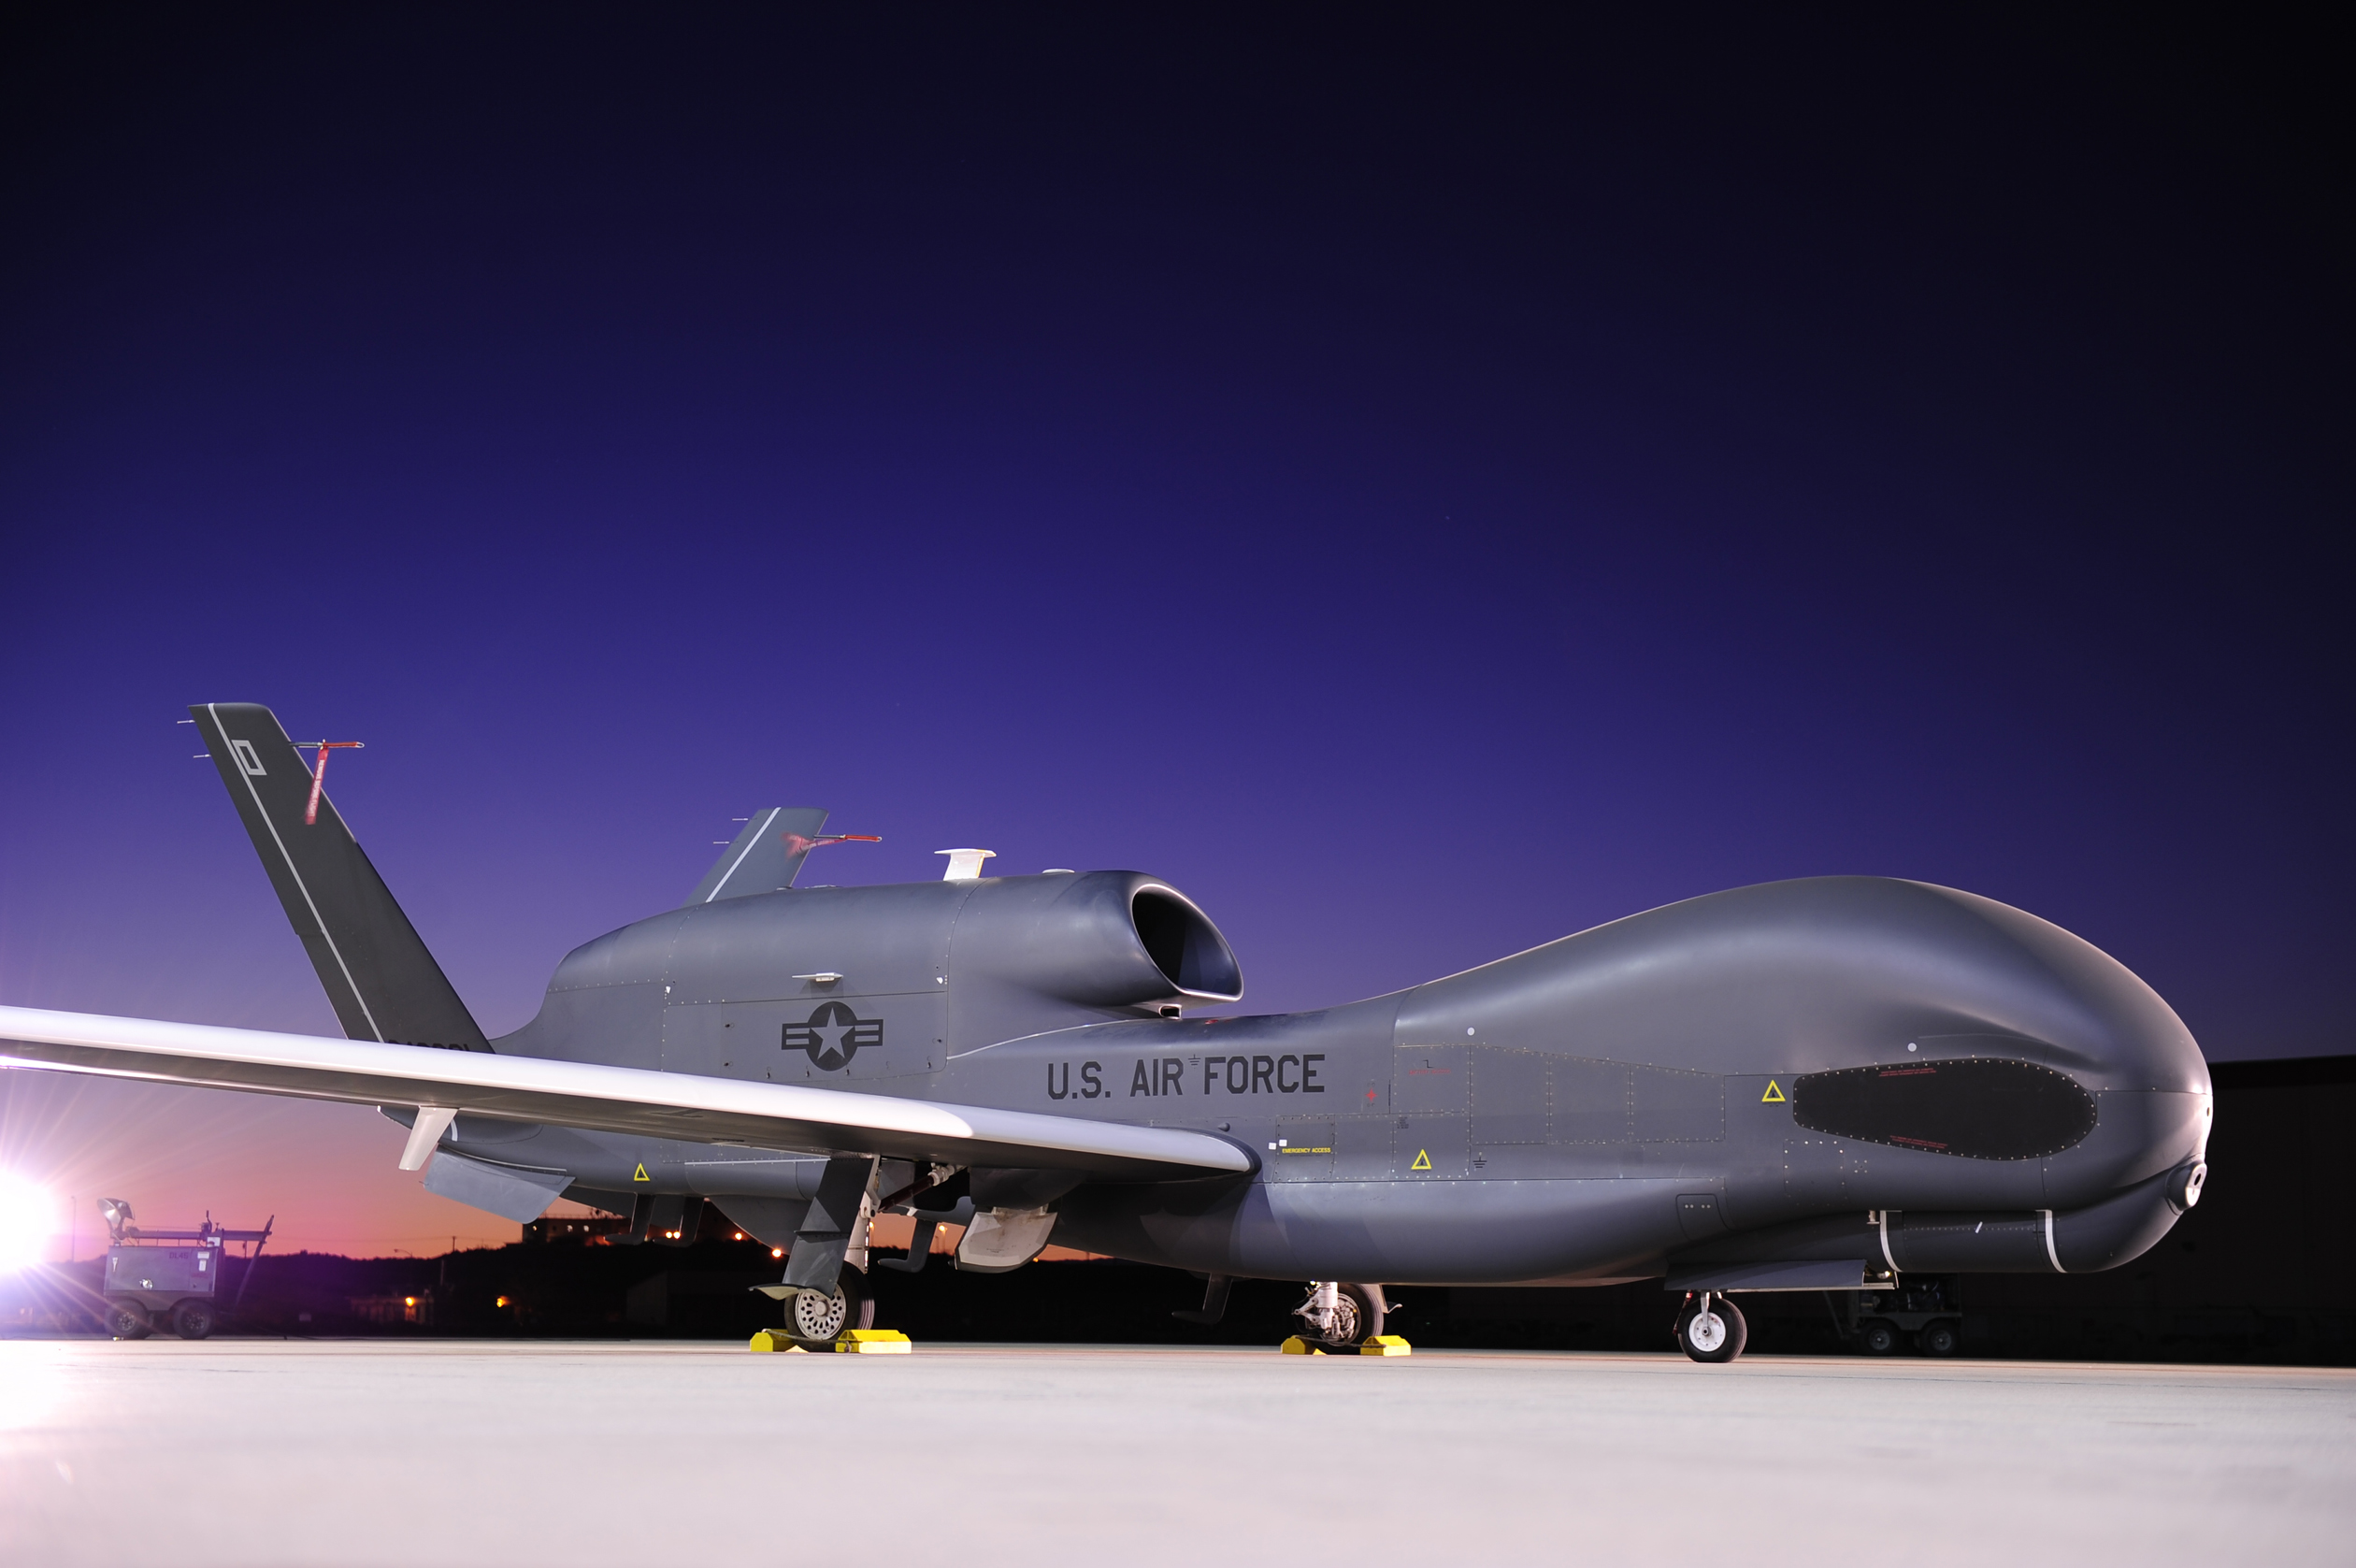
\includegraphics[width=7.7cm] {PaperFigures/globalhawk}}
%		\subfigure []{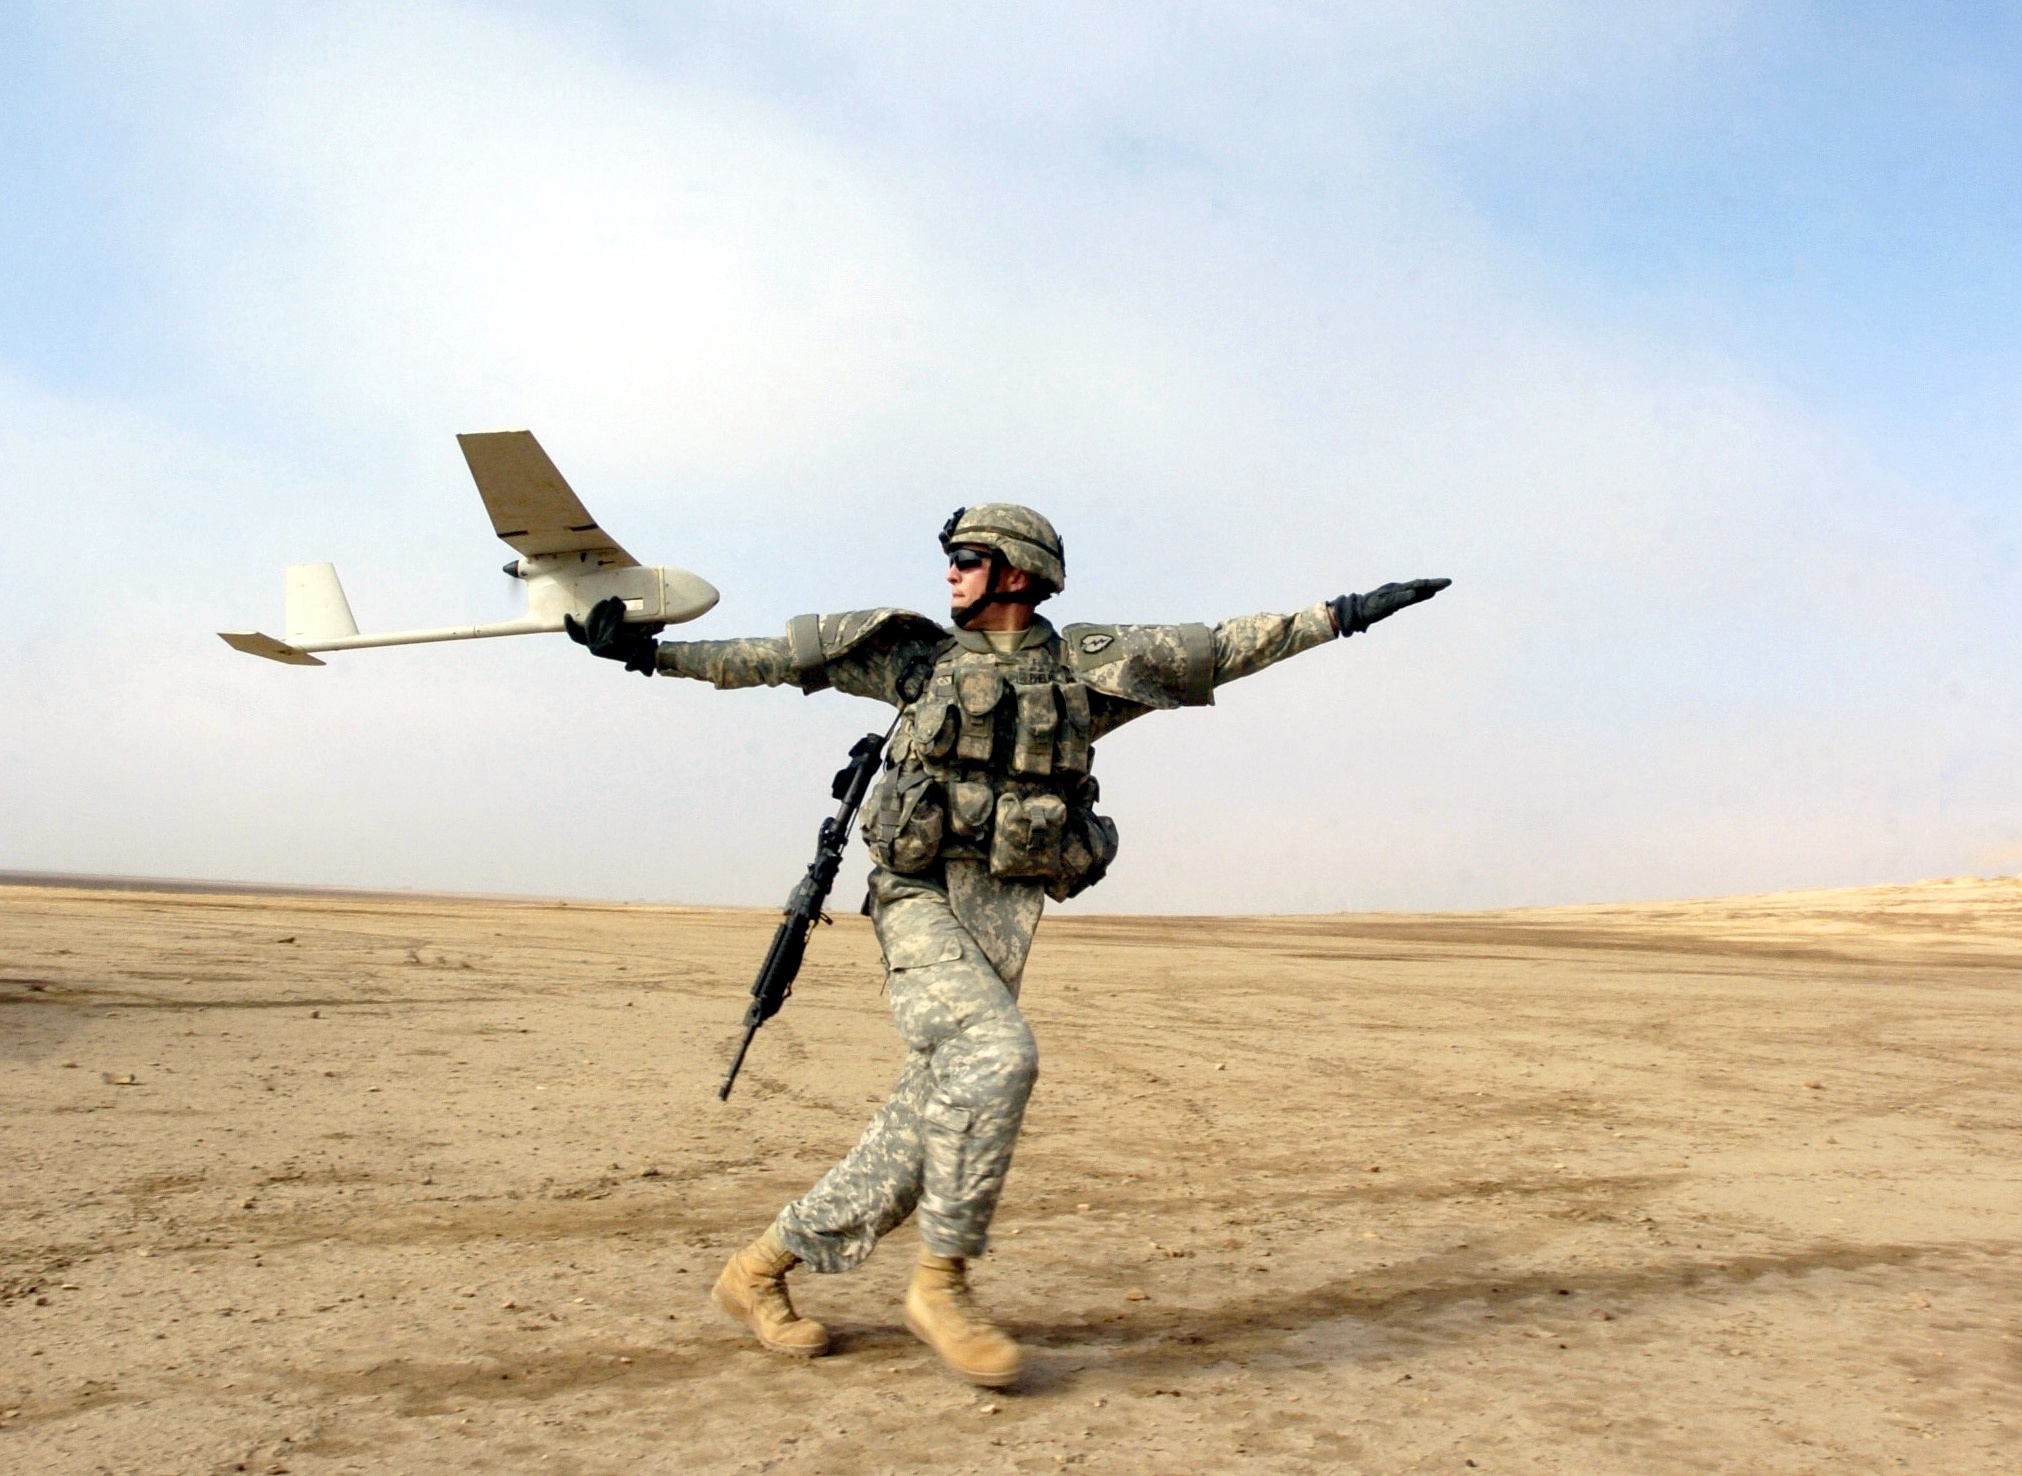
\includegraphics[width=7cm] {PaperFigures/handlaunched}}
%		\hspace*{0mm}
%	\end{subfigmatrix}
%	\caption{Global Hawk and Hand Launched Fixed Wing UAV}
%	\label{fig:fixedwings}
%\end{figure}
%
%
%
%
%
%Both large and hand-launched UAVs operate by using path planning, navigation, guidance, and control algorithms depicted in Figure \ref{fig:ngcflow}. Most UAV tasks can be framed as path following problems such as waypoint navigation or loitering. The UAVs path planner is responsible for generating a flyable path from the current state to the desired state while avoiding known obstacles. Guidance systems are responsible for producing guidance commands to the low level controller that guide the UAV towards the desired path. Navigation systems are responsible for estimating the state of the UAV to provide feedback to both guidance and control loops. For more detail on navigation, guidance, and control systems, refer to section \ref{NGC}. Each of the navigation, guidance, and control sub systems are typically not evaluated independently and must be integrated into a complete system to evaluate the performance as a whole. The most common ways to measure the performance of a UAV system are tracking error with respect to the desired path and control effort. Next, common UAV modeling techniques will be discussed.
%
%%Both large and hand-launched UAVs operate under the same basic principle consisting of navigation, guidance, and control depicted in Figure \ref{fig:ngcflow}. The desired path to be flown is passed to a guidance algorithm whose purpose is to produce guidance ocmmands consumable by the low level-control system that puts the UAV on the desired path. Navigation systems are responsible for estimating the state of the UAV to provide feedback to both guidance and control loops. For more detail on NGC systems, refer to section \ref{NGC}. Each of the NGC sub systems are typically not evaluated independently and must be integrated into a complete NGC system to evaluate th performance as a whole. The most common ways to measure the performance of a UAV system are tracking error with respect to the desired path and control effort.
%
%\begin{figure}[]
%	\centering
%	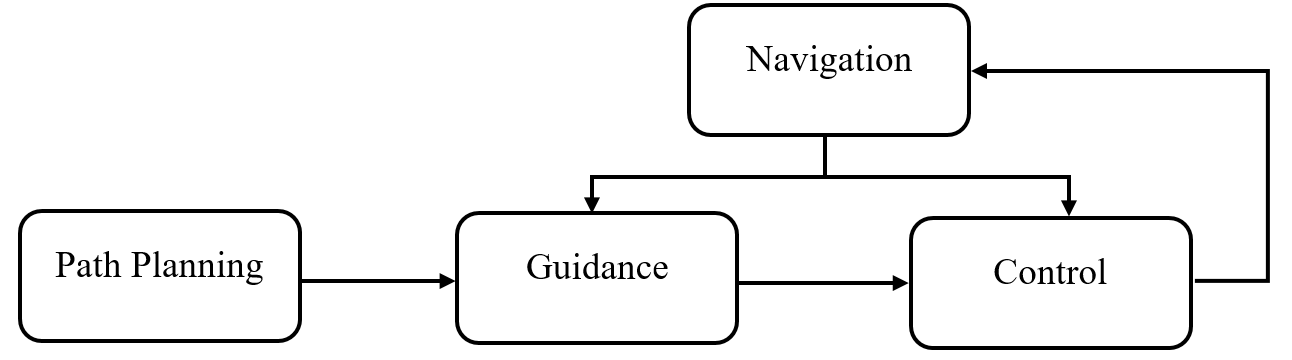
\includegraphics[width=0.7\linewidth]{PaperFigures/ngcFlow}
%	\caption{}
%	\label{fig:ngcflow}
%\end{figure}
%
%
%
%\subsection{Modeling}
%% Modeling of fixed wing UAVs is often simplified
%% High fidelity models are complex because they are high-order and non-linear
%% The 6 degree of freedom crafts only have 4 degrees of controllable freedom resulting in state coupling which also complicates the models
%% High order non-linear models can be simplified when developing control systems that accurately capture the dynamics of the UAV
%% Beyond the control aspect of UAVs, the high order non-linear models are not always necessary. It is common in literature to simplify complex non-linear dynamics of a fixed wing UAV by implementing a 2D Dubins vehicle model \cite{chen_tracking_2009} \cite{liang_tangent_2017} \cite{nelson_cooperative_2005} \cite{griffiths_vector_2006} \cite{jung_unmanned_2016}. When simplified kinematics are used when developing navigation and guidance systems, it is assumed that there already exists a low level control loop that maintains vehicle stability and performs according to the kinematic model in Equations \ref{dubinsx}-\ref{dubinsy}.
%%
%
%Accurate models of fixed wing UAVs tend to be high order, coupled, non-linear systems that can be difficult to solve for. The complexity is due to the fact that a fixed UAV has 6 degrees of freedom with only 4 degrees of control and has non-linear aerodynamic external forces. Models can be linearized and simplified when designing control systems, but still maintain high complexity and require significant effort to implement. Beyond the control aspect of UAVs, the high order non-linear models are not always necessary. It is common in literature to simplify complex non-linear dynamics of a fixed wing UAV by implementing a 2D Dubins vehicle model \cite{chen_tracking_2009} \cite{liang_tangent_2017} \cite{nelson_cooperative_2005} \cite{griffiths_vector_2006} \cite{jung_unmanned_2016}. When simplified kinematics are used when developing navigation and guidance systems, it is assumed that there already exists a low level control loop that maintains vehicle stability and performs according to the kinematic model in Equations \ref{dubinsx}-\ref{dubinsy}.
%
%
%
%
%%The fixed wing UAV is a 6 degree of freedom (DOF) system with four degrees of control consisting of pitch, roll, yaw, and thrust. Change in the control variables is done by actuating the elevator (pitch), ailerons (roll), rudder (yaw), and propeller or jet (thrust). Due to the under actuation and complex non-linear dynamics of the UAV, high fidelity models tend to be high order and non-linear. High order non-linear models can be linearized and simplified to be used in low level control systems to maintain vehicle stability. Beyond the control aspect of UAVs, the high order non-linear models are not always necessary. It is common in literature to simplify complex non-linear dynamics of a fixed wing UAV by implementing a 2D Dubins vehicle model \cite{chen_tracking_2009} \cite{liang_tangent_2017} \cite{nelson_cooperative_2005} \cite{griffiths_vector_2006} \cite{jung_unmanned_2016}. When simplified kinematics are used when developing navigation and guidance systems, it is assumed that there already exists a low level control loop that maintains vehicle stability and performs according to the kinematic model in Equations \ref{dubinsx}-\ref{dubinsy}. 
%
%
%The position of the vehicle at any point in 2D Cartesian space is defined as $(x,y)$ and the velocity of a vehicle in each axis is defined as $(\dot{x},\dot{y})$.
%
%\begin{equation}
%\label{dubinsx}
%\dot{x} = V\cos(\theta)
%\end{equation}
%\begin{equation}
%\label{dubinsy}
%\dot{y} = V\sin(\theta)
%\end{equation}
%
%
%The heading of the vehicle $\theta$ is most frequently used as the input $\boldsymbol{u} = \theta$. To more closely represent the dynamics of a fixed wing, constraints are given to the velocity $V$ and turning rate $\dot{\theta}$. 
%
%
%
%\begin{equation}\label{minVel}
%V \geq V_{stall}
%\end{equation}
%\begin{equation}\label{headingRate}
%-\dot{\theta}_{max} \leq \dot{\theta} \geq \dot{\theta}_{max}
%\end{equation}
%
%The devices that are assumed to be in control of the UAV when designing guidance and navigation systems are called autopilots or flight controllers, which will be discussed briefly in the next section. 
%
%
%\subsection{Autopilot and Ground Station}
%
%%%%%%
%% Fixed wings will rarely be flown without some supplementary ground support
%% UAS - consists of the UAV itself, ground station, and transmitter
%% Ground station acts as a high level command interface for programming mission objectives such as waypoint navigation
%% Ground station is used to interface with autopilot for configurations
%% Ground station can be used to collect data
%% Transmitter allows a pilot to take direct control of the craft in case of an energency
%% Transmitter allows a pilot to take direct control 
%
%% What are autopilots and ground stations
%% Autopilots
%% Ground stations
%% Transmitters
%
%Autopilots and ground stations work together to configure vehicle settings, exchange high-level mission objectives, and collect data. The autopilot is a software and hardware package that brings navigation, guidance, and control techniques to realization. A typical autopilot system is depicted in Figure \ref{fig:pixhawk}, consisting of a hard shell protecting sensors with numerous input and output connectors for power, servo actuation, and communication. Major responsibilities for a autopilot are  maintaining vehicle stability, turning high level commands into low level control effort, and transmitting data to ground stations.
%
%
%
%%The autopilot is a software and hardware package that brings navigation, guidance, and control techniques to realization. A typical autopilot system is depicted in Figure \ref{fig:pixhawk}, consisting of a hard shell protecting sensors with numerous input and output connectors for power, communication, and servo actuation. The flight controller is responsible for several major tasks including maintaining vehicle stability, turning high level commands into low level control effort, and recording and transmitting data to ground stations. Autopilots accomplish these tasks by implementing several layers of algorithms consisting of navigation, guidance, and control which will be discussed next.
%
%
%\begin{figure}[h!]
%	\centering
%	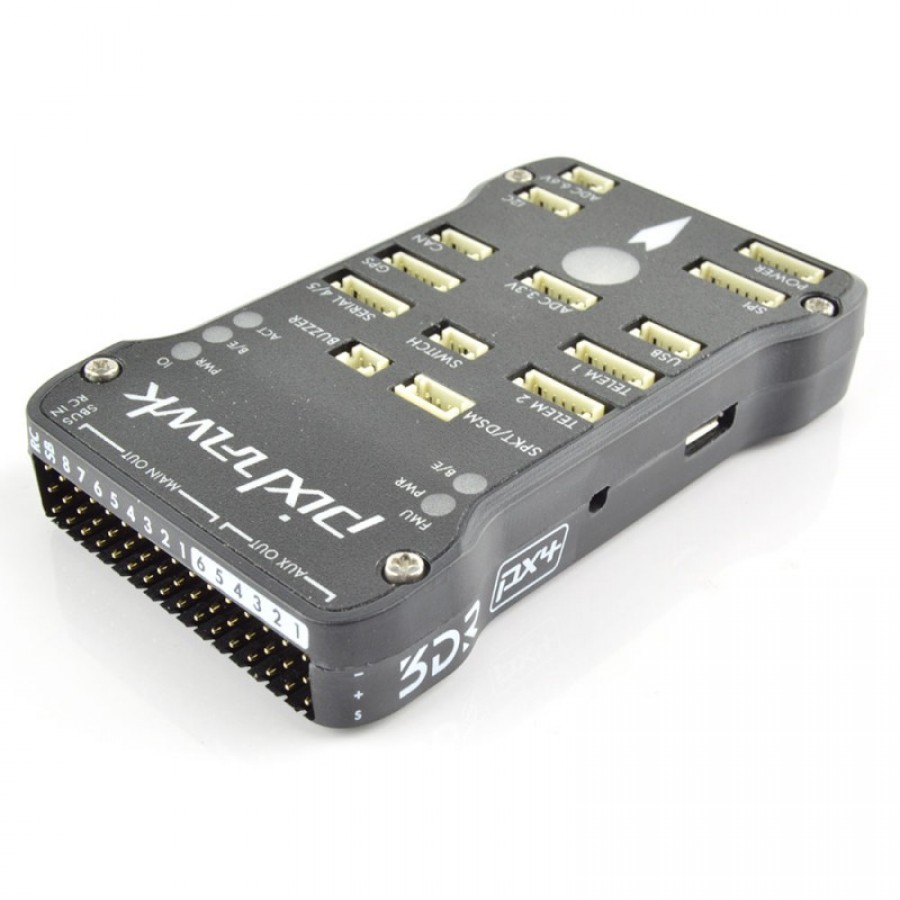
\includegraphics[width=8cm]{PaperFigures/pixhawk}
%	\caption{Pixhawk Flight Controller}
%	\label{fig:pixhawk}
%\end{figure}
%
%
%Ground stations provide an interface for configuring vehicle settings such as cruising velocity and safety protocols. High level mission objectives for waypoint navigation, path following, and loitering are programmed and sent from the ground station to the autopilot. Data collected by the autopilot can also be relayed to the ground station for real time mission updates and for diagnosing problems. 
%
%\begin{figure}
%	\centering
%	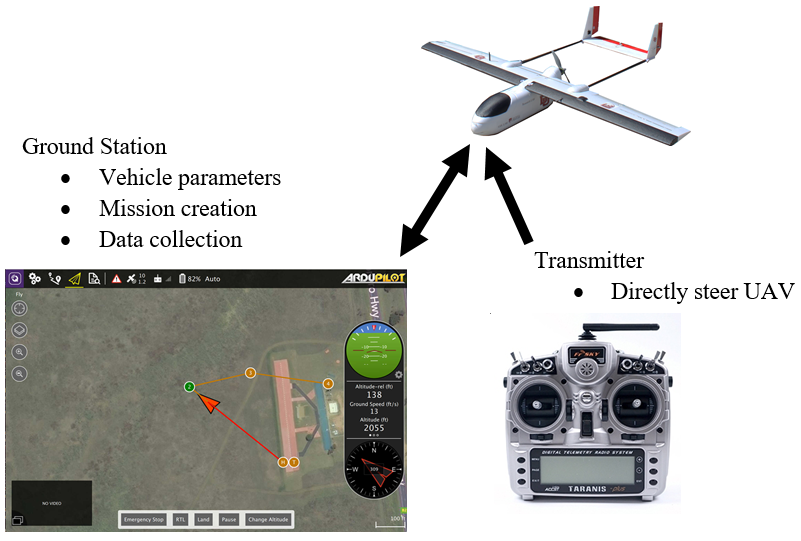
\includegraphics[width=10cm]{PaperFigures/groundUAVTransmitter}
%	\caption{}
%	\label{fig:grounduavtransmitter}
%\end{figure}
%In the event that manual control is required, a transmitter can be used to directly control actuation of the control surfaces on the aircraft. An overview of the autopilot, ground station, and transmitter system is shown in Figure \ref{fig:grounduavtransmitter}.
%
%
%
%
%
%\section{Navigation, Guidance and Control} \label{NGC}
%\subsection{Introduction to NGC}
%Nearly all of the systems that go into an autopilot system for a fixed wing UAV can be put under the category of Navigation, Guidance, or Control (NGC). Traditionally, NGC could be thought of separate but equally important algorithm layers that aid an autopilot in accomplishing a given task. Navigation is the study of measuring, filtering, and estimating the state of a vehicle. Guidance produces a commanded state based on high level requests from a path planner or user. Control maintains vehicle stability while attempting to achieve the state commanded by the high level guidance system. Lately, the lines between guidance and control have become less clear as the systems become more integrated with each other, resulting in more complex capabilities. Continuing with the convention in literature, navigation will be discussed as a separate unit while guidance and control will be discussed simultaneously. Guidance and control will be discussed as a single system and two commonly researched algorithms, potential and vector field methods, will be discussed.
%
%\subsection{Navigation}
%
%Navigation is the study of measuring the position and attitude of the UAV for the purposes of building guidance and providing feedback for the low level control system. Modern flight controllers contain a package of sensors called an Inertial Measurement Unit (IMU) which consists of a 3-axis accelerometer, gyroscope, compass, and barometer. The accelerometer and gyroscope are measured to determine the translational and angular acceleration of the craft. The compass measures heading, and the barometer measures air pressure which is correlated to altitude. IMUs are best for determining the attitude of a UAV but are not used to determine local position due to high noise levels and susceptibility to drift. GPS or motion capture are commonly used to determine local position of a UAV. One of the major challenges in navigation is the noise and uncertainty in sensor measurements. Filters are used to fuse information and provide more accurate estimates of the vehicles position and rate of change. A popular method for filtering and estimating navigation data is done through some variety of a Kalman filter which is a recursive probability method that provides an improved estimation as more information becomes available. The estimates determined by the navigation system are passed to guidance and control systems.
%
%
%\subsection{Guidance and Control}
%
%%Need more citations on traditional guidance systems for path following to add to the discussion
%Guidance and control have traditionally been separate systems, but as the need for UAVs to perform complex tasks increases, so does the complexity of the control systems. A common high level request provided to a UAV is to follow an arbitrary path which can be done with traditional controls \cite{zhao_curved_2017}. A control system for following a moving path was developed in \cite{oliveira_moving_2016}, which was successful at reducing the tracking error in simulation and real flight tests. To accomplish path following of a mobile path, the control law becomes complex and less intuitive. 
%
%%Needs a better transition and explaination of the control system presented in oliveira 
%%Another argument can be made for the distinction between the methods - PF works well for singular point seeking and VF is path seeking
%Instead of relying on complex control laws, there has been much research on methods that combine guidance and control.  Two categories will be discussed consisting of potential field and vector field methods. In literature, the two methods have been seen used interchangeably. In the work presented, potential field is in reference to a gradient potential converging to a local minimum while vector field is in reference to a space of vectors whose integral lines converge and follow a path. It can be argued that vector fields are essentially a potential field, but for organizational purposes, they will be referred to as completely different methods. 
%
%\subsection{Potential Field}
%
%
%%%%%%%%%%%
%Potential field was first introduced as a real-time robotic manipulator algorithm for obstacle avoidance \cite{khatib_real-time_1986}. The potential field algorithm represents a robots workspace as a gradient potential of attractive and repulsive artificial forces that drive the robot to a desired goal. Goals are given the lowest potential and act as attractive forces. Obstacles have high potential and act as repulsive forces. A simple example is depicted in Figure \ref{fig:pfobstacle} consisting of an initial state, a goal, and a single obstacle. The initial state of the robot is at the edge of a gradient where the potential is maximum. In the lowest part of the gradient a goal exists at the global minimum. Obstacles are added to the potential field, but have limited effect due to a decay function.
%
%\begin{figure}[h!]
%	\centering
%	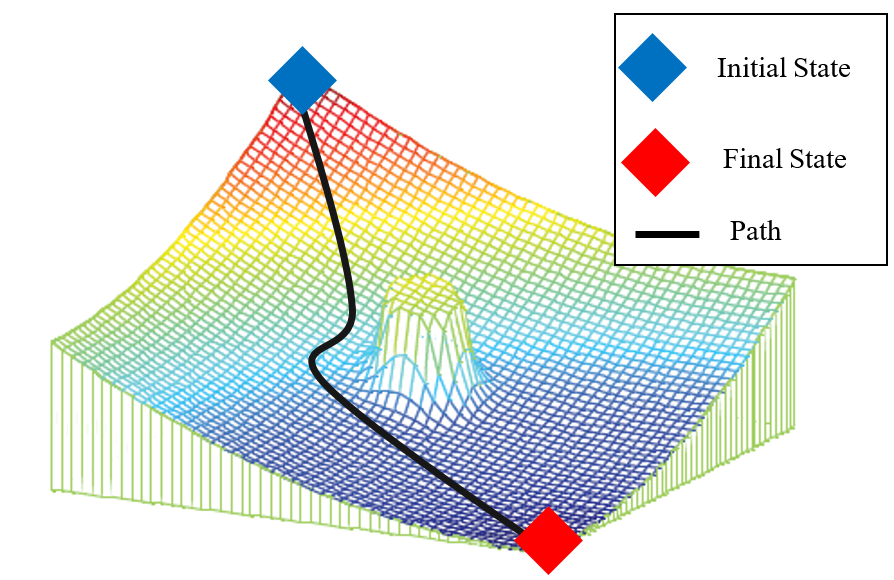
\includegraphics[width=7cm]{PaperFigures/pfObstacle}
%	\caption{Single Obstacle Potential Field Gradient \cite{liu_virtual-waypoint_2016}}
%	\label{fig:pfobstacle}
%\end{figure}
%
%Potential field is unique in that path planning, trajectory planning, and control are lumped into a single system \cite{rimon_exact_1992}. Transition from an initial state to a goal state traditionally occurred by executing three steps consisting of path planning, trajectory planning, and control. Path planning dealt with finding an obstacle free path from an initial state to a goal state. Trajectory planning time parametrized the obstacle free path with some high level vehicle constraints considered. Lastly, control attempts to reduce the tracking error with respect to the reference trajectory. Combining the three motion planning steps into a single algorithm has been shown to be computational inexpensive \cite{goerzen_survey_2010}. 
%
%As pointed out in \cite{borenstein_real-time_1990}, robots using potential field are susceptible to local minimum. Encountering a local minimum prevents the robot from continuing down the gradient and into the global minimum because equilibrium has been reached prematurely. Figure \ref{fig:pfLocalMin} demonstrates local minimum by adding several obstacles into a goal field. Several methods have been developed to mitigate the effects of local minimums as pointed out in \cite{goerzen_survey_2010} through the use of navigation functions. Local minimum produced as a result of closely spaced obstacles as shown in Figure \ref{fig:pfLocalMin} have been addressed by grouping obstacles together into a cluster \cite{liu_virtual-waypoint_2016}.
%
%\begin{figure}[h]
%	\begin{subfigmatrix}{2}% number of columns
%		\centering
%		\subfigure []{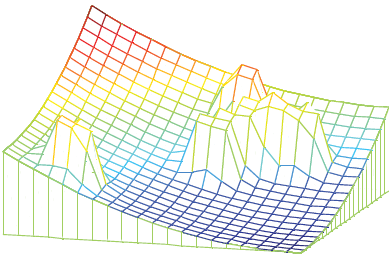
\includegraphics[width=7cm] {PaperFigures/pfObstacleLocalMin}}
%		\subfigure []{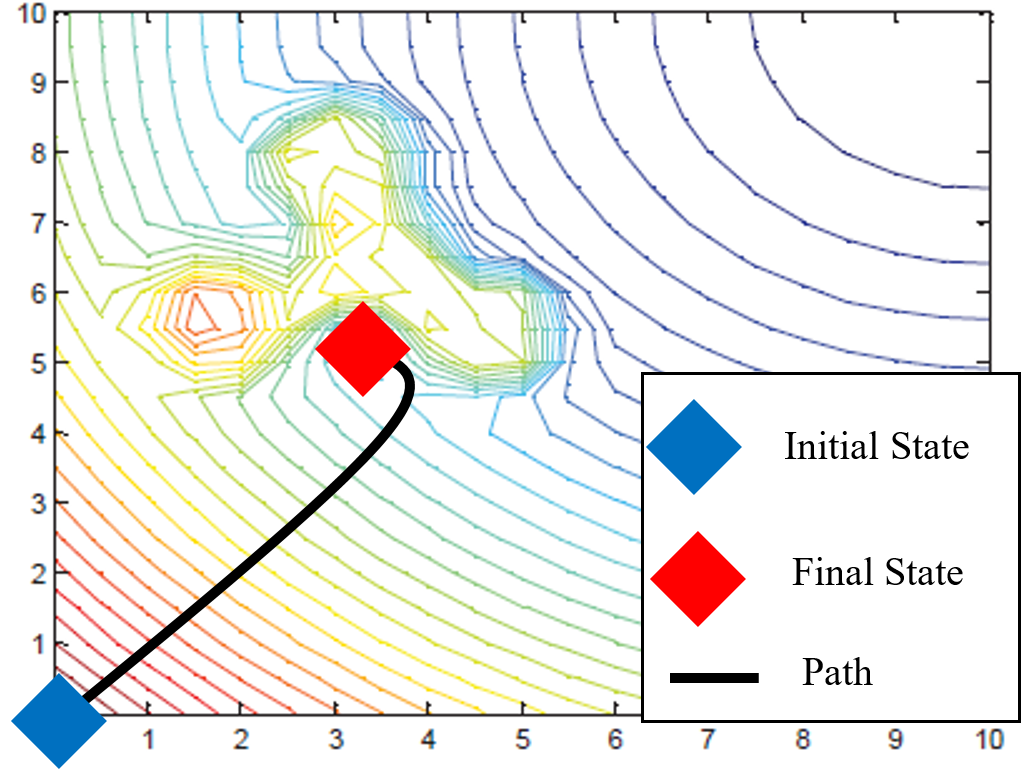
\includegraphics[width=7cm] {PaperFigures/pfObstacleLocalMinTopology}}
%		%		\hspace*{1cm}
%	\end{subfigmatrix}
%	\caption{Potential Field Local Minimum \cite{liu_virtual-waypoint_2016}}
%	\label{fig:pfLocalMin}
%\end{figure}
%
%Several methods have been developed to mitigate the effects of local minimums as pointed out in \cite{goerzen_survey_2010} through the use of navigation functions. Local minimum produced as a result of closely spaced obstacles as shown in Figure \ref{fig:pfLocalMin} have been addressed by grouping obstacles together into a cluster \cite{liu_virtual-waypoint_2016}. Grouping obstacles addresses the risk of local minima before forming the potential field. If local minima are encountered after the field is generated, additional forces can be applied to push the robot away from the local minima. 
%
%\begin{figure}[H]
%	\centering
%	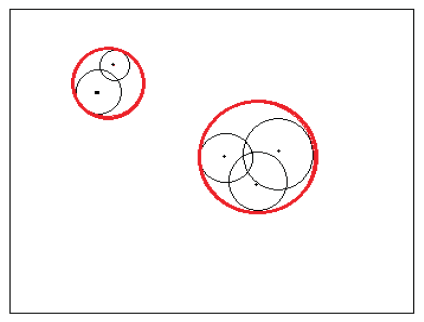
\includegraphics[width=5cm]{PaperFigures/obstacleClustering}
%	\caption{Obstacle Clustering \cite{liu_virtual-waypoint_2016}}
%	\label{fig:obstacleclustering}
%\end{figure}
%
%Potential fields ability to avoid obstacles and combine path planning, trajectory planning, and control into a single system while being computationally inexpensive makes it an attractive option for many robotic systems. Fixed wing UAVs must maintain a minimum forward velocity and cannot converge to a single point, making potential field difficult to implement.  
%
%%Several methods have been developed to mitigate the effects of local minima as pointed out in \cite{goerzen_survey_2010}
%
%
%
%%Potential field is a real-time robotic manipulator algorithm that distributes the task of goal seeking and obstacle avoidance among multiple layers of control \cite{khatib_real-time_1986}. The robot's workspace is represented as a gradient potential of attractive and repulsive artificial forces that drive the robot to a desired state. Goals are represented as an attractive force while obstacles provide a repulsive force. The potential field is constructed by modeling the robots motion in terms of Lagrangian mechanics shown in Equation \ref{LeeMotion}. The Lagrangian is defined as the difference in kinetic energy $T(x,\dot{x})$ and potential energy $U(x)$ in a system. The goal of the system imparts a potential $U_{xd}$ while obstacles impart a repulsive potential $U_o$. 
%%
%%\begin{equation}\label{LeeMotion}
%%\frac{d}{dt} \left(\frac{\partial L}{\partial \dot{x}}\right) - \frac{\partial L}{\partial x} = F
%%\end{equation}
%%
%%\begin{equation}\label{lagrange}
%%L(x,\dot{x}) = T(x,\dot{x}) - U(x)
%%\end{equation}
%%
%%\begin{equation}\label{potential}
%%U_{art}(x) = U_{xd} + U_o(x)
%%\end{equation}
%%
%%Potential field has been shown to be successful at driving a robot from an initial state to a goal state while avoiding obstacles by taking the path of least action formed by the gradient. One of the weaknesses of potential field identified early on is the methods susceptibility to local minima, preventing the robot from reaching the desired global minima, or goal state \cite{koren_potential_1991}. Local minima can be avoided in the potential field method if navigation functions are used \cite{goerzen_survey_2010}.\\
%%
%%Potential field is useful for point-to-point guidance and control which is often the task of UAVs traveling to waypoints, however it is often desired for a UAV to converge to and follow a path. 
%
%%%%%%%%%%% Additional points and clarification needed here before moving on
%%
%% Address navigation functions
%% Re-read Goerzens review article and understand the scope of PF to a better degree
%% Improve the transition to vector field
%%		- Potential fields have proven to be useful for point-to-point navigation, however lack the framework for one of the common applications for fixed wing UAVs, path following
%%
%%
%
%
%
%
%
%
%\subsection{Vector Field}
%
%Converging and following a path instead of a point is more applicable to fixed wing UAVs and has been accomplished through the use of vector fields which will be discussed next.
%
%Path following  
%
%Vector field is a continuous guidance technique that provides heading commands that asymptotically converges and follows a path. 
%
%% intro sentence
%% What is vector field
%% Why is it useful
%% what methods will be discussed
%
%Several methods have been developed to generate vector fields that converge to and follow paths. Histogram virtual force field (VFF) breaks the workspace into discrete cells that contain information in regards to the certainty of the presence of an obstacle \cite{borenstein_real-time_1990} \cite{borenstein_vector_1991}. Cells containing an obstacle apply an artificial guidance force away from the cell. Goals apply a global attractive force that drive the robot towards the desired state. The resultant guidance vector for the VFF method is the sum of the contributions of obstacle repulsive cells and the globally attractive goal. Lyapunov and navigation functions have been successfully used to provide guidance for converging to and following a path. Nelson et al. developed a method for generating a vector field that converges to and follows a path for line and circular primitives \cite{nelson_cooperative_2005}. Sinks, dead zones, and singularities were avoided when constructing more complex flight paths from the primitives by only allowing a single field to be active at any time. A vector field construction method for curved paths was presented in \cite{griffiths_vector_2006} by extending Nelson's method. Elliptical paths have been generated by from primitives by applying coordinate transformations to the field \cite{frew_lyapunov_nodate}.
%
%
%Vector fields have many advantages to traditional guidance. UAVs often encounter disturbances in the form of wind which can be difficult to plan for. In the event a UAV encounters wind disturbances and is pushed off course, the field will drive the vehicle back on course \cite{de_marina_guidance_2017}. In addition to path following, vector field has been used to track a moving target in 3D \cite{miao_orthogonal_2016}. When the location of the target is unknown, loitering about an uncertain target can be achieved by building a circular vector field and applying a linear coordinate transformation to form an elliptical loiter based on the uncertainty in targets position estimate \cite{frew_cooperative_2007}. 
%
%
%%
%% 3D Vector field 
%% \cite{meenakshisundaram_vector_2010}
%%
%%
%%
%
%- Following curved paths in a constant wind \cite{griffiths_vector_2006}
%
%
%%%%%%% Points to make for vector field
%%
%% - Disturbance rejection (wind)
%% - Well suited for unplanned obstacle avoidance
%% - Many applications are best described as path following instead of singular point convergence like potential field
%% - Standoff tracking of uncertain targets
%%
%%
%
%Another method for constructing a vector field is by forming integral curves that converge at the intersection of surfaces \cite{goncalves_artificial_2009}. 
%
%- construct an n-dimensional vector field by forming integral curves that converge at the intersection of surfaces
%- Field is a result of the sum of 3 terms
%- Convergence
%- Circulation
%- Time varying\\
%
%
%% Note, modify the field equation to what jay has in his paper
%\begin{equation}\label{gonFieldeq}
%\boldsymbol{u} = G\nabla_qV+H\wedge_{i=1}\nabla_q\alpha_i - M(\alpha)^{-1}\boldsymbol{a}(\alpha)
%\end{equation}
%
%- Define all variables
%- u is the resulting 2x1 vector
%- Gradient
%- $alpha_i$ is a surface function
%- Wedge product simplifies to cross product in 2d
%- G, H, L scalar weighting quantities 
%- The intersection of the surfaces represents a path to converge and follow
%- Cylinder and plane example
%
%
%\begin{figure}[h]
%	\centering
%	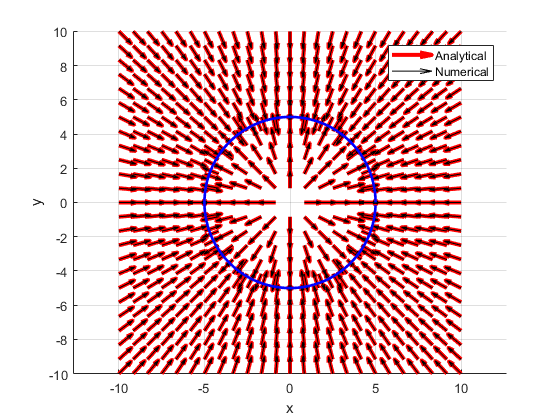
\includegraphics[width=0.7\linewidth]{PaperFigures/convergence}
%	\caption{Convergence}
%	\label{fig:convergence}
%	
%\end{figure}
%
%\begin{figure}[h]
%	\centering
%	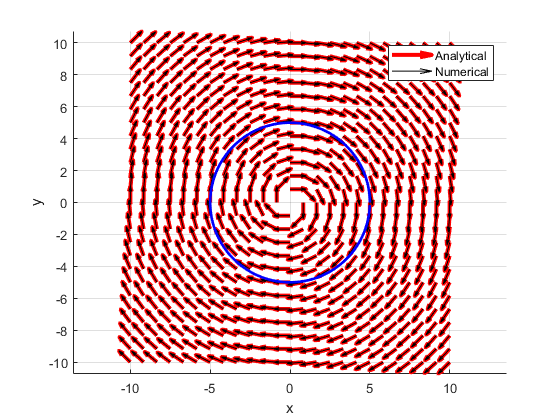
\includegraphics[width=0.7\linewidth]{PaperFigures/circulation}
%	\caption{Circulation}
%	\label{fig:circulation}
%\end{figure}
%
%\begin{figure}[h]
%	\centering
%	\includegraphics[width=0.7\linewidth]{"PaperFigures/time varying"}
%	\caption{Time Varying}
%	\label{fig:time-varying}
%\end{figure}
%
%
%\begin{figure}[h]
%	\centering
%	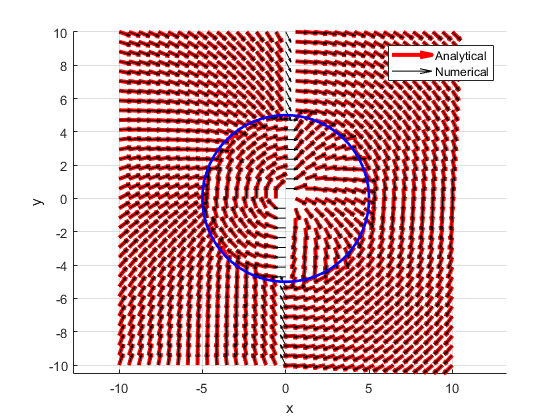
\includegraphics[width=0.7\linewidth]{PaperFigures/total}
%	\caption{Total Field}
%	\label{fig:total}
%\end{figure}
%
%\begin{itemize}
%	\item Cooperative Standoff Tracking of Uncertain moving targets (2007, Frew)
%	\item VF usefulness extended to loitering about an uncertain target
%	\item Lyapunov vector field generation for a circular loiter
%	\item Linear transformation applied to stretch the field into an ellipse shape
%\end{itemize}
%
%
%
%\section{Literature Review Summary}